%% Copyright 1998 Pepe Kubon
%%
%% `two.tex' --- 2nd chapter for thes-full.tex, thes-short-tex from
%%               the `csthesis' bundle
%%
%% You are allowed to distribute this file together with all files
%% mentioned in READ.ME.
%%
%% You are not allowed to modify its contents.
%%

%%%%%%%%%%%%%%%%%%%%%%%%%%%%%%%%%%%%%%%%%%%%%%%%%
%
%     Chapter 2   
%
%%%%%%%%%%%%%%%%%%%%%%%%%%%%%%%%%%%%%%%%%%%%%%%%

\chapter{Background, Data Model, Datasets and Statistical Models}
\label{chap:three}

In this chapter we first provide an introduction to object-relational data model, which is one of the main data models for structured data and has been used to represent our data throughout this dissertation. 
%Section~\ref{sec:other} reviews relevant approaches from different data models, the most common atomic object model where data is represented by a single data matrix and structured data models using the XML, SQL, and OLAP formats.
In section \ref{sec:synthetic} we discuss three synthetic and two real-world datasets that have been designed to evaluate the performance of our outlier detection methods. In section~\ref{sec:otherStat} we review the necessary background on statistical models that have been employed in this dissertation.  Section \ref{sec:eval} explains the evaluation techniques we have utilized to examine the outlier detection methods that will be introduced in chapter~\ref{chap:four} and~\ref{chap:five}.


%In section~\ref{sec:data models}, % we introduce few commonly used data models that have been employed in outlier detection task.
%we review relevant approaches from different data models, the most common atomic object model where data is represented by a single data matrix and structured data models using the XML, SQL, and OLAP formats.
% We then provide an introduction to object-relational data model which is one of the main data models for structured data and has been used to represent our data throughout this dissertation. 
 %We also briefly introduce other types of structured data models that have been used in outlier detection work in literature.   %In section \ref{sec:object} of this chapter we provide an introduction to Object-relational data model which is one of the main data models for structured data. We used object-relation model to represent our data throughout this dissertation~\cite{Koller1997}.
% Section \ref{sec:object} explains Object-Relational Data model that has been used to represent data in the next chapters. 
  %in the remaining chapters of this dissertation. 
 %\section{Background}
 
 	\section{Object-relational Data Model}
 	% To our knowledge, our work is the first model-based method tailored for object-relational data.
 	 %Object-relational data is one of the main data models for structured data~\cite{Koller1997}. 
 	 The main 
 	 characteristics of objects that we utilize in this dissertation are the following:
 	 \begin{enumerate}
 	 	\item {\em Object Identity.} Each object has a unique identifier that is the same across contexts. For example, a player has a name that identifies him in different matches.
 	 	\item  {\em Class Membership.} An object is an instance of a class, which is a collection of similar objects. Objects in the same class share a set of attributes. For example, van Persie is a player object that belongs to the class striker, which is a subclass of the  class player.
 	 	\item{\em Object Relationship.} Objects are linked  to other objects. Both objects and their links have attributes. A common type of object relationship is a component relationship between a complex object and its parts.
 	 \end{enumerate}
 	 
 	 For example, a match links two teams, and each team comprises a set of players for that match. A difference between relational and vectorial data is that an individual object is characterized not only by a list of attributes but also by its links and by attributes of the object linked to it. We refer to the substructure comprising this information as the {\em object data}. Object-relational data can be represented as a network as shown in Figure~\ref{fig:graphical_represetnaion}.
 	 
 	 \textbf{Example} A query for computing object data for Arsenal includes the selection condition $TeamID=Arsenal$. Note that object data features all the data of the object as well as the data from more complex objects within that object.
 	 
 	 
 	 %To implement this, for each target object, we form 
 	 The appropriate \textbf{object data table} is formed from the population data table by restricting the relevant first-order variable to the target object. 
 	 For example, the object database for target Team $\it{Wigan Athletic}$ 
 	 forms a subtable of the data table of Table~\ref{table:data-chapt3} that contains only rows where 
 	 TeamID = $\it{WA}$; see Table~\ref{table:individual-chapt3}. In database terminology, an object database is like a view centered on the object.
 	 
 	 
 	 
 	 \subsection{Notation and Definition}
 	 
 	 %	\subsubsection{Relational Data}
 	 	
 	 	
 	 	
 	 	
 	 	%We apply the learn-and-join algorithm (LAJ), which is the state-of-the-art Bayes net learning method for relational data. The LAJ algorithm takes as input a relational database and outputs a Bayes net using the functor notation due to Poole \cite{Poole2003}. We briefly review this notation.
 	 	
 	 	%\paragraph{Functor Terms} 
 	 	We adopt a term-based notation for combining logical and statistical concepts~\cite{Poole2003,Kimmig2014}.
 	 	A functor is a function or a predicate symbol. Each functor has a set of values (constants) called the \textbf{domain} of the functor. The domain of a \textbf{predicate} is $\{\true,\false\}$. Predicates are usually written with uppercase Roman letters, other terms with lowercase letters.
 	 	A predicate of arity at least two is a \textbf{relationship} functor. Relationship functors specify which objects are linked. Other functors represent \textbf{features} or \textbf{attributes} of an object or a tuple of objects (i.e., of a relationship).
 	 	A \textbf{population} is a set of objects. 
 	 	A \textbf{term} is of the form $f(\term_{1},\ldots,\term_{k})$ where $\functor$ is a functor %(either a function symbol or a predicate symbol) 
 	 	and each $\term_{i}$ is a first-order variable or a constant denoting an object. A term/literal/formula is \textbf{ground} if it contains no first-order variables, otherwise it is a first-order term. In the context of a statistical model, we refer to first-order terms as \textbf{Parametrized Random Variables} (PRVs) \cite{Kimmig2014}. 
 	 	%A term whose range are the truth values $\{\true,\false\}$ is a \textbf{predicate}. 
 	 	%Predicates are usually written with uppercase Roman letters, other term with lowercase letters.
 	 	%The grounding concept represents moving from the population-level  to the object level. 
 	 	A \textbf{grounding} replaces each first-order variable in a term/literal/formula by a constant, the result is a ground term. A grounding may be applied simultaneously to a set of terms.  A relational database $\D$ specifies the values of all ground terms. %, which can be listed in data tables. 
 	 	%In machine learning terminology, the data tables are contingency tables that represent sufficient statistics or event counts.
 	 	
 	 	Consider a joint assignment (also known as conjunctive formula or conjunction in logic)
 	 	$P(\Features = \set{\nodevalue})$ of values to a set of PRVs $\Features$ . The {\em grounding space} of the PRVs is the set of all possible grounding substitutions, each applied to all PRVs in $\Features$. The {\em count} of groundings that satisfy the assignment with respect to a database $\D$ is denoted by $\grounds_{\D}(\Features = \set{\nodevalue})$. The \textbf{database frequency} $P_{\D}(\Features = \set{\nodevalue})$ is the grounding count divided by the number of all possible groundings. 
 	 	%, that is, the size of the grounding space.
 	 	
 	 	\paragraph{Example} \label{sec:example}
 	 	%
 	 	The Opta dataset represents information about Premier League data %\cite{opta-original} 
 	 	(Sec.~\ref{sec:real-world-data}). 
 	 	%Using the functor notation, the data
 	 	%format can be represented as follows. 
 	 	The basic populations are teams, players, and matches with 
 	 	corresponding first-order variables $\team, \player, \match$. As shown in Table~\ref{table:data-chapt3}, the groundings count can be visualized in terms of a groundings table ~\cite{Schulte2012}, also called a universal schema~\cite{Riedel2013}. 
 	 	%Table~\ref{table:data} specifies values for some ground terms. 
 	 	The first three column headers show first-order variables ranging over different populations. The remaining columns represent terms. Each row represents a single grounding and the values of the ground terms are defined by the grounding.
 	 	%Table~\ref{table:counts} illustrates grounding counts. 
 	 	In terms of the grounding table, the grounding count of a joint assignment is the number of rows that satisfy the conditions in the joint assignment. In the network view representation of data, grounding count represents the number of subgraphs that satisfy a given conjunction as shown in Figure~\ref{fig:graphical_represetnaion}.  The database frequency is the grounding count divided by the total number of rows in the groundings table. Counts are based on the 2011-2012 Premier League Season. We count only groundings $(\it{team},\it{match})$ such that $\it{team}$ plays in $\it{match}$. Each team, including Wigan Athletics, appears in 38 matches. The total number of team-match pairs is $38 \times 20 = 760$.
 	 	\paragraph{Example} Figure~\ref{main:a-chap3} shows an example database. The ground literal\\ \centerline{$(\it{ShotEff(\P,\M)} = Low) \{\P$\textbackslash$ 123,\M$\textbackslash$ 1\}=(\it{ShotEff}(123,1)=Low)$}\\ evaluates as true in this database. For the grounding count we have\\ \centerline{$\grounds_{\D}(\it{ShotEff(\P,\M)} = Low) \{\P$\textbackslash$ 123\}) = 2.$}
 	 	
 	 	\begin{figure}
 	 		\centering
 	 		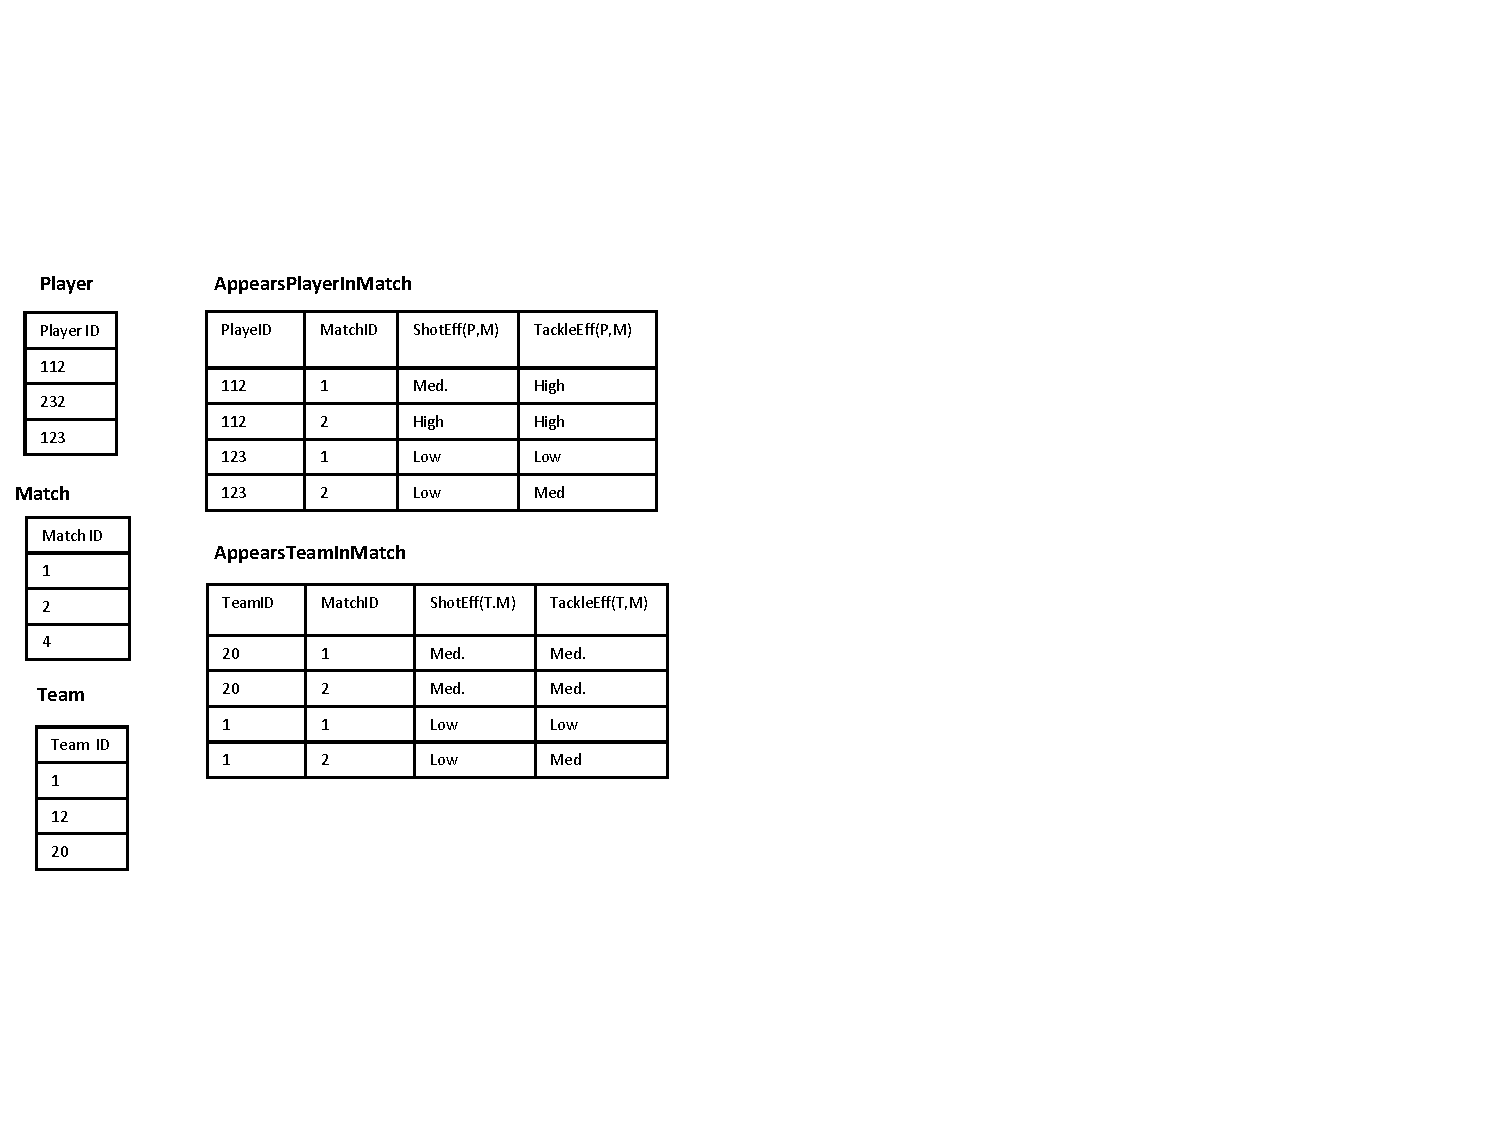
\includegraphics[width=0.6\textwidth] {figures/databasefigure.pdf}
 	 		\caption{An example database
 	 			\label{main:a-chap3}}
 	 	\end{figure}
 	 	%Examples of terms include the following. 
 	 	
 	 	%\begin{itemize}
 	 	%\item $\it{Appears\_Player}(\P,\M)$ indicates whether a player appeared in a match.
 	 	%\item $\it{Appears\_Team}(\T,\M)$ indicates whether a team played in a match.
 	 	%\item $\it{Team}(\P)$ returns the team of a player.
 	 	%\item $\it{Result}(\T,\M)$ denotes the result of a team in a match (win or lose).
 	 	%\item $\it{ShotEff}(\T,\M)$ denotes the shot efficiency of a team in a match (number of successful shots on target, per total number of shots).
 	 	%\item $\it{TimePlayed}(\P,\M)$ denotes the total time that a player played in a match.
 	 	%\end{itemize}
 	 	
 	 	
 	 	%\begin{table}[htbp]
 	 	%\caption{Examples of terms in the soccer dataset.}
 	 	%\centering
 	 	%\resizebox{1\textwidth}{!}{
 	 	%\begin{tabular}{|c|p{5cm}|}
 	 	%\hline
 	 	%Term&Meaning\\ \hline
 	 	%$\it{Appears\_Player}(\P,\M)$ & indicates whether a player appeared in a match.\\ \hline
 	 	%$\it{Appears\_Team}(\T,\M)$&indicates whether a team played in a match.\\ \hline
 	 	%$\it{Team}(\P)$& returns the team of a player.\\ \hline
 	 	%$\it{Result}(\T,\M)$ &denotes the result of a team in a match (win or lose).\\ \hline
 	 	%$\it{ShotEff}(\T,\M)$ &denotes the shot efficiency of a team in a match (number of successful shots on target, per total number of shots).\\ \hline
 	 	%$\it{TimePlayed}(\P,\M)$& denotes the total time that a player played in a match.\\ \hline
 	 	%\end{tabular}}
 	 	%\label{table:terms}
 	 	%\end{table}
 	 	
 	 	\begin{table}[htbp]
 	 		\caption{Sample population data table (Soccer). \label{table:data-chapt3}}
 	 		\centering
 	 		\resizebox{1\textwidth}{!}{
 	 			\begin{tabular}{|c|c|l|c|c|c|c|}
 	 				\hline
 	 				\multicolumn{1}{|l|}{MatchId \match} &
 	 				TeamId \team & PlayerId \player& \multicolumn{1}{l|}{First\_goal(\player,\match)} 
 	 				& \multicolumn{1}{l|}{TimePlayed(\player,\match)} & 
 	 				\multicolumn{1}{l|}{ShotEff(\team,\match)}&result(\team,\match) \\ \hline
 	 				117 & WA & McCarthy & 0 & 90 & 0.53&\it{win}\\ \hline
 	 				148 & WA & McCarthy & 0 & 85 & 0.57&\it{loss}\\ \hline
 	 				15 & MC & Silva & 1 & 90 & 0.59&\it{win}\\ \hline
 	 				\ldots& \ldots &\ldots&\ldots&\ldots&\ldots&\\
 	 			\end{tabular}}
 	 			\caption{Sample object data table, for team $\team = \it{WA}$. \label{table:individual-chapt3}}
 	 			\resizebox{1\textwidth}{!}{
 	 				\begin{tabular}{|c|c|l|c|c|c|c|}
 	 					\hline
 	 					\multicolumn{1}{|l|}{MatchId \match} &
 	 					TeamId $\team = \it{WA}$ & PlayerId \player& \multicolumn{1}{l|}{First\_goal(\player,\match)} 
 	 					& \multicolumn{1}{l|}{TimePlayed(\player,\match)} & 
 	 					\multicolumn{1}{l|}{ShotEff(\it{WA},\match)}&result(\it{WA},\match) \\ \hline
 	 					117 & WA & McCarthy & 0 & 90 & 0.53&\it{win}\\ \hline
 	 					148 & WA & McCarthy & 0 & 85 & 0.57&\it{loss}\\ \hline
 	 					\ldots& WA &\ldots&\ldots&\ldots&\ldots&\\
 	 				\end{tabular}}
 	 			\end{table}
 	 			
 	 			
 	 			
 	 			
 	 			%[The object database is an individual-centered representation \cite{Flach1999a}. move to related work.]
 	 			
 	 			%\begin{table} 
 	 			%	\captionsetup{singlelinecheck=off}
 	 			%			\caption[.]{\label{table:counts}Example of Grounding Count and Frequency for the conjunction \begin{displaymath} \it{passEff(T,M)=hi}, shotEff(T,M)=high, Result(T,M)=1.\end{displaymath}}
 	 			%			\centering
 	 			%			\resizebox{1\textwidth}{!}{
 	 			%				\begin{tabular}{|c|c|c|}
 	 			%					\hline
 	 			%					Database&Count or $\#_{D}(\Features = \set{\nodevalue})$&Frequency or $P_{D}(\Features = \set{\nodevalue})$\\\hline
 	 			%					Population&76& $76/760=0.10$\\\hline
 	 			%					Wigan Athletics&7&$7/38=0.18$\\\hline
 	 			%		
 	 			%					%Synthetic&40&280\\ \hline
 	 			%				\end{tabular}}
 	 			%			\end{table}
 	 			\begin{table} 
 	 				\caption{Example of grounding count and frequency in the Premier League, for the conjunction $\it{passEff(T,M)=high}$, $\it{shotEff(T,M)=high}$,$ \it{Result(T,M)=win}$.\label{table:counts}}
 	 				\centering
 	 				\resizebox{1\textwidth}{!}{
 	 					\begin{tabular}{|c|c|c|}
 	 						\hline
 	 						Database&Count or $\#_{D}(\Features = \set{\nodevalue})$&Frequency or $P_{D}(\Features = \set{\nodevalue})$\\\hline
 	 						Population&76& $76/760=0.10$\\\hline                                                                               	
 	 						Wigan Athletics&7&$7/38=0.18$\\\hline
 	 						
 	 						%Synthetic&40&280\\ \hline
 	 					\end{tabular}}
 	 				\end{table}
 	 				
 	 				 	 			\begin{table} 
 	 				 	 				\caption{Instances of the conjunction: $\it{passEff(T,M)=high}$, $\it{shotEff(T,M)=high},$ $\it{Result(T,M)=win}$ in the network representation of Figure~\ref{fig:graphical_represetnaion}.\label{table:counts}}
 	 				 	 				\centering
 	 				 	 				\resizebox{1\textwidth}{!}{
 	 				 	 					\begin{tabular}{|c|c|c|c|c|c|}
 	 				 	 						\hline
 	 				 	 						Team&Player&MatchID&$\it{shotEff(T,M)}$&$\it{passEff(T,M)}$&$\it{Result(T,M)}$\\\hline
 	 				 	 						Manchester United&Javier Hernandez&119&high&high&win\\\hline
 	 				 	 						Manchester United&Anderson&119&high&high&win\\\hline
 	 				 	 						
 	 				 	 						%Synthetic&40&280\\ \hline
 	 				 	 					\end{tabular}}
 	 				 	 				\end{table}
 	 				 	 				
 	 				 	 					
 	 				 	 					\begin{figure}[t]
 	 				 	 						\centering
 	 				 	 						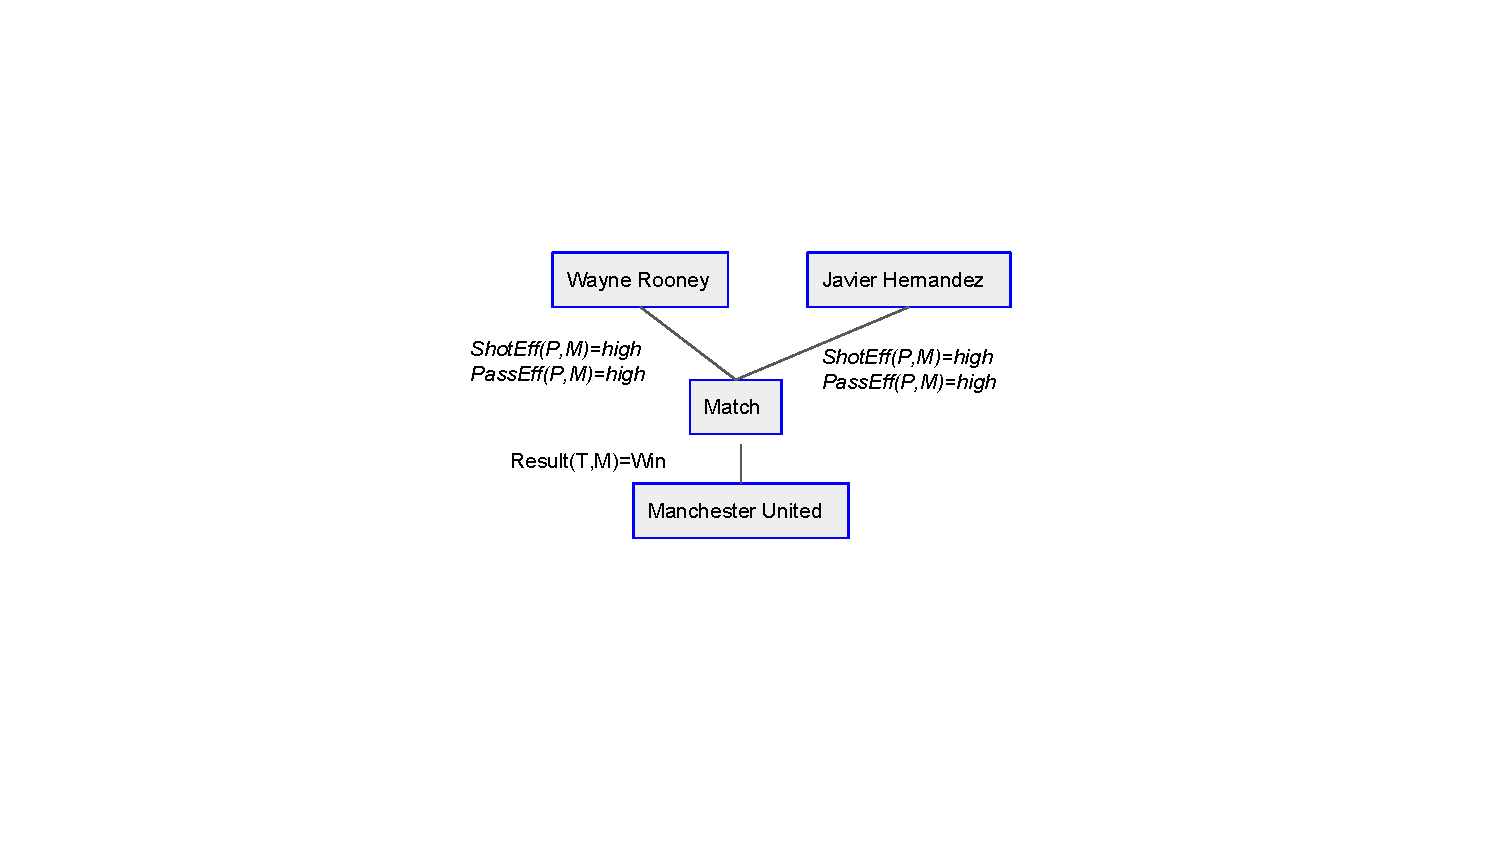
\includegraphics[width=0.7\textwidth] 
 	 				 	 						{figures/instancesofNetwork.pdf}
 	 				 	 						\caption{In the network representation, We have shown two instances of the conjunction: $\it{passEff(T,M)=hi}$, $\it{shotEff(T,M)=hi},$ $\it{Result(T,M)=win}$. We use the conjunctions to define subgraphs.  
 	 				 	 							%We show only the Markov blanket of the Results node to simplify. 
 	 				 	 							\label{fig:graphical_represetnaion}
 	 				 	 						}
 	 				 	 					\end{figure}
 	 				
 	 				%\begin{table} 
 	 				%	\captionsetup{singlelinecheck=off}
 	 				%			\caption[.]{\label{table:counts}Example of Grounding Count and Frequency for the conjunction \begin{displaymath} \it{passEff(T,M)=hi}, shotEff(T,M)=high, Result(T,M)=1.\end{displaymath} Counts are based on the 2011-2012 Premier League Season. We count only groundings $(\it{team},\it{match})$ such that $\it{team}$ plays in $\it{match}$. Each team, including Wigan Athletics, appears in 38 matches. The total number of team-match pairs is $38 \times 20 = 760$.
 	 				%			\label{MetricComputation}}
 	 				%			\centering
 	 				%			\resizebox{1\textwidth}{!}{
 	 				%				\begin{tabular}{|c|c|c|}
 	 				%					\hline
 	 				%					Database&Count or $\#_{D}(\Features = \set{\nodevalue})$&Frequency or $P_{D}(\Features = \set{\nodevalue})$\\\hline
 	 				%					Population&76& $76/760=0.10$\\\hline
 	 				%					Wigan Athletics&7&$7/38=0.18$\\\hline
 	 				%		
 	 				%					%Synthetic&40&280\\ \hline
 	 				%				\end{tabular}}
 	 				%				
 	 				
 	 
% 	 \section{Other Data Models}\label{sec:other}
% 	  In this section, we review some of the data models that have been previously used to represent the data for outlier detection task.
% 	  \begin{enumerate}
% 	  	
% 	  	\subsection{Attribute Vector Data Model}
% 	  		\textit{a) Attribute Vector Data Model:}
% 	  	
% 	  	By far most work on outlier detection considers atomic objects with flat feature vectors.
% 	  	, or nonhierarchical structures like time series. 
% 	  	This leads to an impedance mismatch: 
% 	  	The required input format for these outlier detection methods is a single data matrix, not a structured dataset. For example, one cannot provide a relational database as input. This mismatch is not simply a question of choosing a file format, but instead reflects a different underlying data model: complex objects with both attributes and component objects vs. atomic objects with attributes only. 
% 	  	
% 	  	It is possible to ``flatten'' structured data by converting it to unstructured feature vectors, for instance by using aggregate functions. 
% 	  	Flattening incurs some loss of information but allows us to apply the many feature vector methods.
% 	  	\cite{Elke2013}. 
% 	  		We evaluated the aggregation approach in this paper by applying three standard methods for outlier detection.
% 	  	for three major approaches to outlier detection: distance-based, density-based, and subspace clustering. 
% 	  	
% 	  	Subspace clustering methods (e.g., \cite{Muller2012,Kriegel2009}) are similar to our work in the sense that they aim to decompose a complex data space. They find complex deviations that are noticeable only in a data subspace. A common approach is to discover datapoints that show unexpected deviations in similar subspaces. Our approach instead develops a joint measure of how dissimilar the target object profile distribution is to the class distribution over the entire data space. Given that object and class distributions are represented by an object-oriented Bayesian network \cite{Koller1997}, the network structure defines subspaces. The joint divergence measure {\em mathematically decomposes} into subspace measures that quantify how dissimilar the target object profile distribution is in the subspaces defined by the network, compared to the class distribution in the same subspace.
% 	  	
% 	  	Work on atomic contextual  outliers \cite{Tang2013} is like ours in that it considers the distinctness of a target individual from a reference class. A reference class is not specified for each object,
% 	  	as a property of the object, 
% 	  	but is constructed as part of outlier detection. 
% 	  	Our work could be combined with a class discovery approach by providing a score of how informative the inferred classes are. 
% 	  	 	\begin{figure}
% 	  	 		\centering
% 	  	 		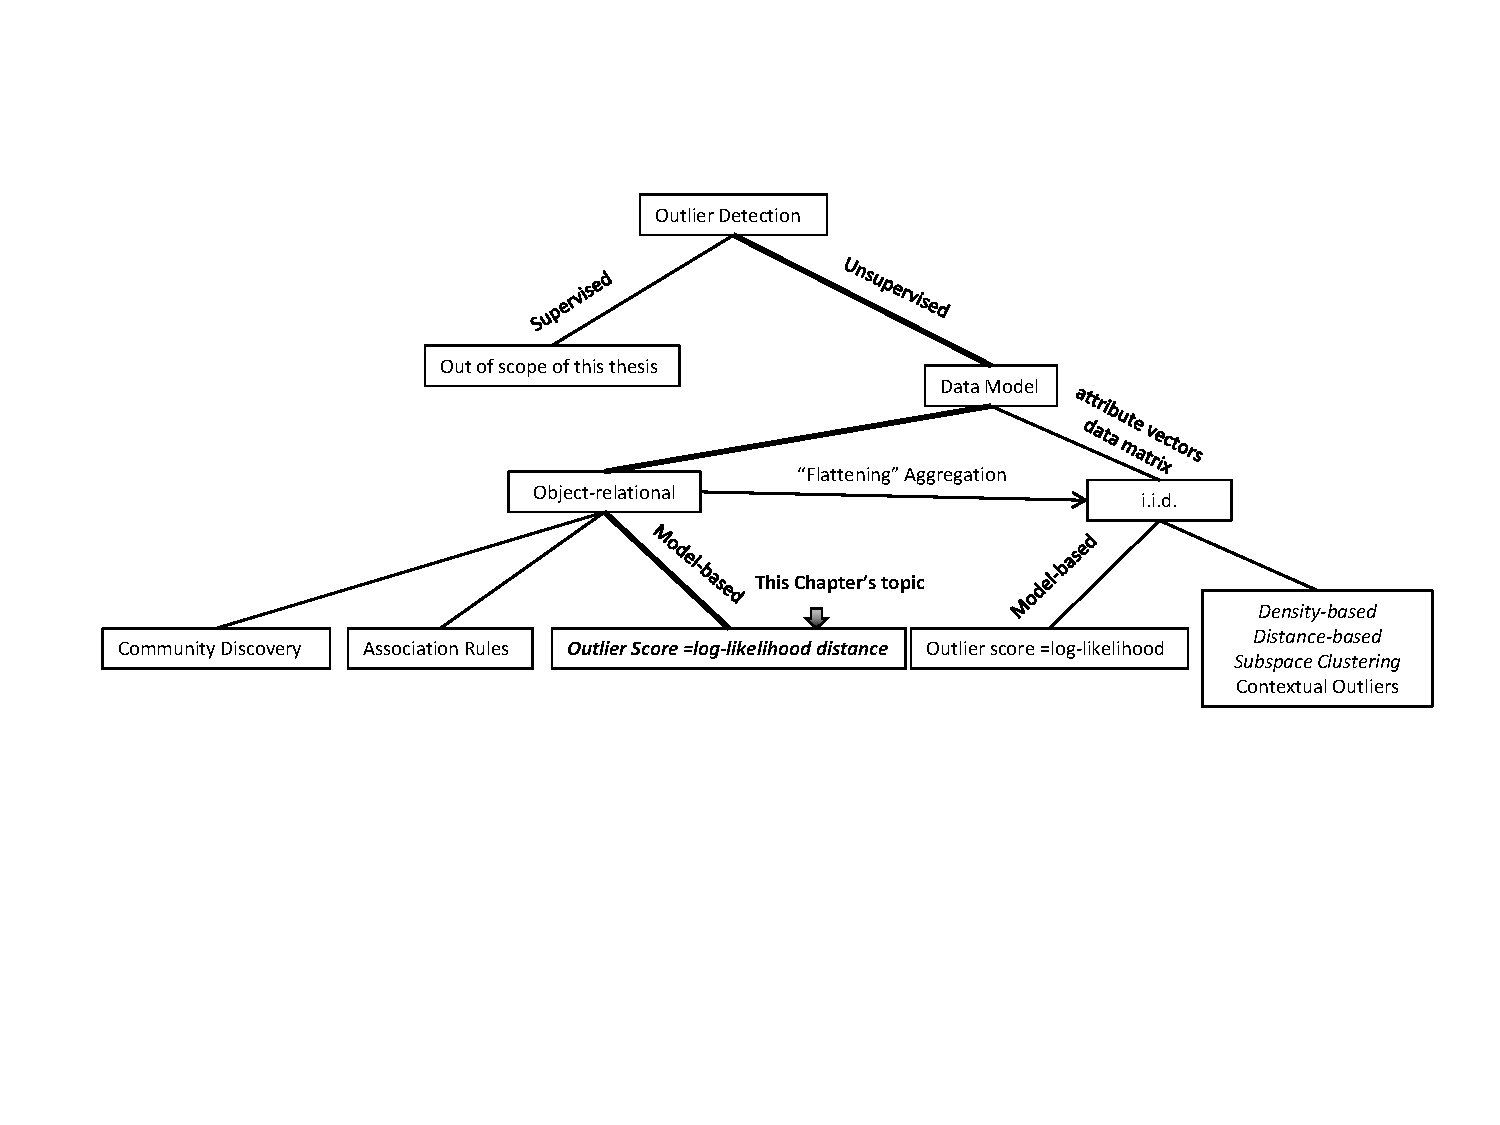
\includegraphics[width=1\textwidth] {figures/novelty-sep.pdf}
% 	  	 		\caption{A tree structure for related work on outlier detection for structured data. A path specifies an outlier detection problem, the leaves list major approaches to the problem. Approaches in italics appear in experiments.
% 	  	 			\label{fig:novelty}}
% 	  	 	\end{figure}
% 	  	\vspace{-5mm}
% 	  	
% 	  	We discuss related techniques in three types of structured data models: SQL (relational), XML (hierarchical), and OLAP (multi-dimensional). 
% 	  	
% 	  	For relational data, many outlier detection approaches aim to discover rules that represent the presence of anomalous associations for an individual or the absence of normal associations \cite{Maervoet2012,Gao2010}. The survey by \cite{Novak2009} unifies within a general rule search framework related tasks such as exception mining, which looks for associations that characterize unusual cases, subgroup mining, which looks for associations  characterizing important subgroups, and contrast space mining, which looks for differences between classes. Another rule-based approach uses Inductive Logic Programming techniques \cite{Angiulli2007}.
% 	  	,Angiulli2009}.
% 	  	While local rules are informative, they are not based on a global statistical model and do not provide a single outlier score for each individual. 
% 	  	
% 	  	A latent variable approach in information networks ranks potential outliers in reference to the latent communities inferred by network analysis \cite{Gao2010}. Our model aggregates information from entities and links of different types, but does not assume that different communities have been identified. 
% 	  	\subsection{Structured Data Models}	%\textit{b) }
% 	  	Koh {\em et al.}~\cite{koh2008} propose a method for hierarchical structures represented in XML document trees. Their aim is to identify feature outliers, not class outliers as in our work. Also, they use aggregate functions to convert the object hierarchy into feature vectors. Their outlier score is based on local correlations, and they do not construct a model.
% 	  	
% 	  	
% 	  	The multi-dimensional data model defines numeric measures for a set of dimensions. 
% 	  	A seminal approach to exploring a multi-dimensional datacube was presented by Sarawagi {\em et al.}~\cite{Sarawagi1998}. 
% 	  	The object and the multi-dimensional data models are similar in the respect that both objects and dimensions are ordered in a hierarchy. However, 
% 	  	The differences in the two data models mean that multi-dimensional outlier detection models~\cite{Sarawagi1998} do not carry over to object-relational outlier detection. (1) The object data model allows but does not require any numeric measures. In our datasets, all features are discrete. Nor do we assume that it is possible to aggregate numeric measures to summarize lower-level data at higher levels.  
% 	  	(2) In scoring a potential outlier object, our method considers other objects {\em both} below and above the target object in the component hierarchy. OLAP exploration methods consider only cells below or at the same level as the target cell. For example, in scoring a player, our method would consider features of the player's team.  
% 	  	Also, our proposed outlier score of an object is not determined by the outlier scores of its components, in contrast to the approach of Sarawagi {\em et al.}~\cite{Sarawagi1998}.
% 	  	 They use values such as the most unusual cell that is below a target cell.
% 	  	(3) Our approach models a joint distribution over features, exploiting correlations among features. Most of the OLAP-based methods consider only a single numeric measure at a time, not a joint model. \\ 
\section{Synthetic Datasets} \label{sec:synthetic}
 
 We generated three synthetic datasets with normal and outlier players using the distributions represented in the three Bayesian networks of Figure~\ref{fig:synthetic-bns}. 
 %The features $F_{1}$ and $F_{2}$ represent two features of players. 
 Each player participates in 38 matches, similar to the real-world data. The main goal of designing synthetic experiments is to test the methods on  easy to detect outliers. Each match assigns a value to each feature $F_i, i =  1,2$ for each player. 
 \begin{description}
 	\item\textbf{High Correlation}  Normal individuals exhibit a strong association between their features, outliers no association. Both normals and outliers have a close to uniform distribution over single features. See Figure~\ref{fig:synthetic-bns}(a).
 	\item\textbf{Low Correlation}  Normal individuals exhibit no association between their features, outliers have a strong association. Both normals and outliers have a close to uniform distribution over single features. See Figure~\ref{fig:synthetic-bns}(b).
 	\item\textbf{Single features}  Both normal and outlier individuals exhibit a strong association between their features. In normals, 90\% of the time, feature 1 has value 0. For outliers, feature 1 has value 0 only 10\% of the time. See Figure~\ref{fig:synthetic-bns}(c).
 \end{description}
 We used the $\it{mlbench}$ package in $\it{R}$ to generate synthetic features in matche and followed these distributions for 240 normal players and 40 outliers. We followed the real-world Opta data in terms of number of normal and outlier individuals. %The scores are used to rank all 280 players. 
 
 \begin{figure*}[htbp]
 	\centering
 	\resizebox{1\textwidth}{!}{
 		\includegraphics%[width=0.3\textwidth] 
 		{figures/figure1kddCropped.pdf}
 	}
 	\caption{Illustrative Bayesian networks. The networks are not learned from data, but hand-constructed to be plausible for the soccer domain. (a) High Correlation;
 		% The outlier distribution misses a correlation that is present in the normal population. The single feature distributions are uniform in both distributions. 
 		(b) Low Correlation;
 		% The outlier object exhibits a correlation that is not present in the normal population. The single attribute distributions are uniform in both distributions.
 		(c) Single Attributes.
 		%Correlations are the same, but the single feature distributions are not.
 		\label{fig:synthetic-bns}}
 \end{figure*}
 
 
 \section{Real-world Datasets} \label{sec:real-world-data}
 In this dissertation, real world data tables are prepared from Opta data~\cite{opta-original} and IMDb~\cite{IMDb-original}.% Our datasets and code are available on-line~\cite{bib:url}.
 Table~\ref{table:Features-chapter3} lists the populations and features. Table~\ref{table:StatsChapter3} shows summary statistics for the datasets. 
 %	
 %	\begin{table}[htbp]
 %		\centering
 %		\resizebox{0.4\textwidth}{!}{
 %			\begin{tabular}{|c|p{5cm}|}
 %				\hline
 %				Individuals & Features\\ \hline
 %				\begin{tabular}{c}Soccer-Player\\per Match \end{tabular} & $\it{TimePlayed}$,$\it{Goals}$,$\it{SavesMade}$,
 %				$\it{ShotEff}$,$\it{PassEff}$,$\it{WinningGoal}$,
 %				$\it{FirstGoal}$,$\it{PositionID}$, $\it{TackleEff}$,$\it{DribbleEff}$,
 %				$\it{ShotsOnTarget}$ \\ \hline
 %				\begin{tabular}{c}Soccer-Team\\per Match \end{tabular} & $\it{Result}$,$\it{TeamFormation}$,$\sum\it{Goals}$,
 %				$\mu\it{ShotEff}$,$\mu\it{PassEff}$,$\mu\it{TackleEff}$, 
 %				$\mu\it{DribbleEff}$. \\ \hline
 %				IMDB-Actor & $\it{Quality}$, $\it{Gender}$ \\ \hline
 %				IMDB-Director & $\it{Quality}$,$\it{avgRevenue}$\\ \hline
 %				IMDB-Movie&$\it{year}$,$\it{isEnglish}$,$\it{Genre}$,$\it{Country}$, $\it{RunningTime}$, $\it{Rating}$ by User\\ \hline
 %				IMDB-User& %$\it{Rating}$,
 %				$\it{Gender}$, $\it{Occupation}$.\\ \hline
 %			\end{tabular}}	
 %			\caption{Attribute Features. $\mu$ = average, $\\sum$ = sum. For relationships please see text.\label{table:Features}}
 %			
 %		\end{table}
 
 
 \begin{table}[htbp]
 	\centering
 	\resizebox{0.6\textwidth}{!}{
 		\begin{tabular}{|c|p{5cm}|}
 			\hline
 			Individuals & Features\\ \hline
 			\begin{tabular}{c}Soccer-Player\\per Match \end{tabular} & $\it{TimePlayed}$,$\it{Goals}$,$\it{SavesMade}$,
 			$\it{ShotEff}$,$\it{PassEff}$,$\it{WinningGoal}$,
 			$\it{FirstGoal}$,$\it{PositionID}$, $\it{TackleEff}$,$\it{DribbleEff}$,
 			$\it{ShotsOnTarget}$ \\ \hline
 			\begin{tabular}{c}Soccer-Team\\per Match \end{tabular} & $\it{Result}$,$\it{TeamFormation}$,
 			$\sum\it{Goals}$,$\mu\it{ShotEff}$,$\mu\it{PassEff}$,
 			$\mu\it{TackleEff}$,$\mu\it{DribbleEff}$. \\ \hline
 			IMDB-Actor & $\it{Quality}$, $\it{Gender}$ \\ \hline
 			IMDB-Director & $\it{Quality}$,$\it{avgRevenue}$\\ \hline
 			IMDB-Movie&$\it{year}$,$\it{isEnglish}$,$\it{Genre}$,$\it{Country}$, $\it{RunningTime}$, $\it{Rating}$ by User\\ \hline
 			IMDB-User& %$\it{Rating}$,
 			$\it{Gender}$, $\it{Occupation}$.\\ \hline
 		\end{tabular}}
 		\caption{Attribute features.% $\mu$ = average, $\\sum$ = sum. For relationships please see text.
 			\label{table:Features-chapter3}}
 		
 	\end{table}
 	\paragraph{Soccer Data} 
 	The Opta data were released by Manchester City. 
 	It lists all the ball actions within each game, by each player, for the 2011-2012 season. 
 	%The data consists of information about the actions of a single player in a given match 
 	%from 2011 to 2012. 
 	Number of goals, passes, fouls, tackles, saves and blocks, and also the position 
 	assigned to a player in a match, are examples of the information associated with each player.
 	%Information about the teams in a season, such as number of home wins, draws or away wins can be extracted by massaging the data. 
 	%[The information can be visualized as a heterogeneous network that links players to teams, and teams to matches. ]
 	For each player in a match, our dataset contains eleven player features.
 	% like $\it{TimePlayed}(\P,\M)$.
 	For each team in a match, there are five features computed as player feature aggregates, as well as the team formation and the result (win, tie, loss). 
 	There are two relationships, $\it{Appears\_Player}(\P,\M)$, $\it{Appears\_Team}(\T,\M)$. 
 	%We store the data in a relational database, with a table for each base population and a table for each relationship.
 	We refer to the Premier League data as the {\em Soccer} dataset.
 	Table~\ref{table:StatsChapter3} shows summary statistics for the datasets. 
 	\begin{table}
 		\centering
 		\resizebox{0.8\textwidth}{!}{
 			\begin{tabular}{|l|l|l|l|} \hline
 				\multicolumn{2}{|c|}{Premier League Statistics}& \multicolumn{2}{|c|}{IMDB Statistics}\\
 				\hline
 				Number Teams&20&Number Movies&3060 \\ \hline
 				Number Players&484&Number Directors&220 \\ \hline
 				Number Matches&380&Number Actors&98690  \\ \hline
 				avg player per match&26.01& avg actor per movie&36.42  \\ \hline
 			\end{tabular} 
 		}
 		\caption{Summary statistics for the IMDb and the Premier League datasets}
 		\label{table:StatsChapter3}
 	\end{table}
 	
 	\paragraph{IMDB Data} 
 	The Internet Movie Database (IMDB) is an on-line database of information related to films, television programs and video games.
 	The IMDB website offers a dataset containing information on cast, crew, titles, technical details and biographies in a set of compressed text files. 
 	We preprocessed the data like, \cite{Peralta2007}, to obtain a database with seven tables, one for each population and one for the three relationships: $\it{Rated}(\user,\movie)$, $\it{Directs}(\director,\movie)$, and $\it{ActsIn}(\actor,\movie)$.
 	
 	%	Table~\ref{table:Features-prime} lists relationships and the number of features. 
 	%					\begin{table}[htbp]
 	%								\caption{Relationships and Example Features in Real-World Datasets.
 	%									%For relationships please see text.
 	%									\label{table:Features}}
 	%						\centering
 	%						\resizebox{0.6 \textwidth}{!}{
 	%							\begin{tabular}{|l|c|l|}
 	%								\hline
 	%								Path/Object Type & \#Attributes&Example\\ \hline
 	%								\begin{tabular}{c}Player-Team-Match \end{tabular} & 11&ShotEff \\ \hline
 	%								\begin{tabular}{c}Team-Match \end{tabular} & 7&TeamFormation \\ \hline\hline
 	%								Actor & 2&Quality \\ \hline
 	%								Director & 2&AvgRevenue\\ \hline
 	%								Movie&5&Genre\\ \hline
 	%								User& 2&Occupation\\ \hline
 	%								User-Movie & 1&Rating \\\hline
 	%								Actor-Movie & 1&Cast\_Position\\\hline
 	%							\end{tabular}}
 	%					
 	%						\end{table}
 	%\footnote{Commented table of relationships and features}
 	%					\begin{LaTeXdescription}
 	%						\item[Soccer Data]
 	%						The Opta data were released by Manchester City. 
 	%						It lists all the ball actions within each game by each player, for the 2011-2012 season.
 	%						\item[IMDb Data]
 	%						The Internet Movie Database (IMDb) is an online database of information related to films, television programs, and video games.
 	%						The IMDb website offers a dataset containing information on cast, crew, titles, technical details and biographies in a set of compressed text files \cite{Peralta2007}.
 	%					\end{LaTeXdescription}
 	
 	%\subsection{Outlier and Contrast Classes.}
 	
 	In real-world data there is no ground truth about which objects are outliers. To address this issue we employ a one-class design: we learn a model for the class distribution, with data from only that class. We then rank all individuals from the normal class, together with all objects from a contrast class treated as outliers, in order to test whether an outlier score recognizes objects from the contrast class as outliers.
 	%		distinguishes objects from the normal class from objects in the contrast class. 
 	Table~\ref{MetricComputation} shows the normal and contrast classes for three different datasets.  In-class outliers are possible, e.g. unusual strikers are still members of the striker class. Chapter~\ref{chap:five} describes a few in-class outliers. In the soccer data we considered only individuals who played more than 5 matches out of a maximum 38. 
 	
 	\begin{table}
 		\caption{Outlier/normal objects in real-world datasets. }
 		\label{MetricComputation}
 		\centering
 		\resizebox{0.5\textwidth}{!}{
 			\begin{tabular}{|c|c|c|c|}
 				\hline
 				Normal&\#Normal&Outlier&\#Outlier\\\hline
 				Striker & 153 & Goalie&22\\ \hline
 				Midfielder & 155 & Striker&74\\ \hline
 				Drama & 197 & Comedy&47\\ \hline
 				%Synthetic&40&280\\ \hline
 			\end{tabular}}
 			
 		\end{table}
 		
 	\section{Statistical Models} \label{sec:otherStat}
 	
 	We use notation and terminology from previous work \cite{Poole2003,Chiang2012,Lippi2011,Domingos2009}. While we do not introduce any new terminology, we combine concepts from different areas, such as propositionalization and log-linear models. 
 	
 	%				\subsection{Predicate Language}
 	%				
 	%				We employ the notation of Chiang and Poole \cite{Chiang2012} for logical syntax, as follows.
 	%				%
 	%				Constants are expressed in lower-case, e.g. $\it{joe}$, and are used to represent individuals. A type is associated with each individual, e.g. $\it{joe}$ is a person. We use $D(\tau)$ to represent a domain of type $\tau$, which is the set of individuals of type $\tau$. A {\em logical variable} is written in upper case. A logical variable is also typed, e.g. $\it{Person}$ denotes some member of $D(\tau)$. A relation is given by 
 	%				$$r : \Omega \rightarrow V_{r}$$
 	%				where $r$ is the name of the relation, $\Omega_{r}=D(\tau_{1})\times \ldots \times D(\tau_{a})$ is the domain of the relation, and $T_{r}=(\tau_{1},\ldots,\tau_{a})$ is the type of the relation. $V_{r}={v_{1},\ldots,v_{k}}$ is the range of the relation. Number $a$ and $k$ are positive integers denoting the {\em arity} and {\em size} of $r$. An {\em atom} is an expression of the form $r(\sigma_{1},\ldots,\sigma_{a})$ where each $\sigma_{i}$ is either a constant or logical variable. If all of $\sigma_{1},\ldots,\sigma_{a}$ are constants, $r(\sigma_{1},\ldots,\sigma_{a})$ is a {\em ground atom}.
 	%				
 	%				A {\em literal} specifies the value of an atom e.g. $r(X_{1},\ldots,X_{a})=v$ where $v \in V_{r}$. A literal is also a {\em formula}. Formulae with multiple literals are formed using connectives $\wedge$ and or $\vee$. Connecting literals using only $\wedge$ forms a {\em conjunctive formula } or {\em conjunction}. A formula that contains no logical variables is a {\em ground} formula.
 	%				%, is a proposition.
 	%				%A {\em disjunctive formula} or {\em disjunction} is formed using only $\vee$. \\
 	%				
 	%				A substitution is a set $\{X_{1} \textbackslash x_{1}, \ldots, X_{k}\textbackslash x_{k}\}$ where $X_{i}$ are distinct logical variables and $x_{i}$ are constants. When applied to a formula $f$, each occurrence of $X_{i}$ in $f$ is replaced with $x_{i}$. We denote the application of a substitution 
 	%				%$\{X_{1} \textbackslash x_{1}, \ldots, X_{k}\textbackslash x_{k}\}$ 
 	%				to $f$ as $f\{X_{1} \textbackslash x_{1}, \ldots, X_{k}\textbackslash x_{k}\}$. 
 	%				Consider a formula $f$ containing logical variables $X_{1}, \ldots,X_{n}$, where each $X_{i}$ has type $\tau_{i}$. The {\em grounding space} of $f$, is the set of all possible grounding substitutions for $f$, given by 
 	%				$$\{\{X_{1}\textbackslash x_{1}, \ldots, X_{n}\textbackslash x_{n}\}:x_{i} \in D(\tau_{i}) \mbox{ for } i=1,\ldots,n\}.$$
 	%				
 	%				%	Given some formula $f$ containing logical variables $X_{1}, \ldots,X_{n}$, where each $X_{i}$ has type $\tau_{i}$, let the domain of $f$ be $\Omega_{f}=D(\tau_{i}\times \tau_{n})$. The {\em substitution space} of $f$, $\Gamma_{f}$, is the set of all possible grounding substitutions for $f$, given by 
 	%				%	$$\Gamma_{f}=\{\{X_{1}\textbackslash x_{1}, \ldots, X_{n}\textbackslash x_{n}\}:(x_{1},\ldots,x_{n})\in \Omega_{f}\}.$$
 	%				
 	%				A \emph{database} $\D$ specifies for each ground literal whether the literal is true in the database or not. A ground conjunction is true in a database if all of its conjuncts are true. The \emph{count} of groundings satisfying formula $\formula$ with respect to a database $\D$ is denoted as $\grounds_{\D}(\formula)$.
 	%	
 	
 	\subsection{Bayesian Network}
 	We adopt  
 	the Parametrized Bayes net (PBN) formalism \cite{Poole2003} that combines Bayes nets with logical syntax for expressing relational concepts. 
 	
 	
 %	\subsubsection{Bayesian Networks}
 	
 	A {\bf Bayesian Network (BN) structure} $\model$ is a directed acyclic graph (DAG)  whose nodes comprise a set of random variables \cite{Pearl1988}. Depending on the context, we interchangeably refer to the nodes  and variables of a BN. Fix a set of variables $\Features = \{\feature_{1},\ldots,\feature_{n}\}$. 
 	%These are attributes of objects, which can and typically do belong to different classes. In statistical terms, each attribute defines a random variable. 
 	The possible values of $\feature_{i}$ are enumerated as $\{\nodevalue_{i1},\ldots,\nodevalue_{i\states_{i}}\}$. The notation $P(\feature_{i} = \nodevalue)\equiv P(\nodevalue)$ denotes the probability of variable $\feature_{i}$ taking on value $\nodevalue$. We also use the vector notation $P(\Features = \set{\nodevalue}) \equiv P(\set{\nodevalue})$ to denote the joint probability that each variable $\feature_{i}$ takes on value $\set{\nodevalue}_{i}$. 
 	
 	
 	The conditional probability parameters of a Bayesian network specify the distribution of a child node given an assignment of values to its parent node. For an assignment of values to its nodes, a BN defines the joint probability as the product of the conditional probability of the child node value given its parent values, for each child node in the network. This means that the log-joint probability can be {\em decomposed} as the node-wise sum
 	
 	\begin{equation} \label{eq:bn}
 	\ln P(\Features = \set{\nodevalue};\model,\parameters) = \sum_{i=1}^{n} \ln \parameter(\set{\nodevalue}_{i}|\set{\nodevalue}_{\parents_{i}})
 	\end{equation}
 	
 	where $\set{\nodevalue}_{i}$ resp. $\set{\nodevalue}_{\parents_{i}}$ is the assignment of values to node $\feature_{i}$ resp. the parents of $\feature_{i}$ determined by the assignment $\set{\nodevalue}$. 
 	%The function $\ln$ is the binary logarithm base 2. 
 	To avoid difficulties with $\ln(0)$, here and below we assume that joint distributions are positive everywhere. Since the parameter values $\parameters$ for a Bayes net define a joint distribution over its nodes, they therefore entail a marginal, or unconditional, probability for a single node. We denote the \textbf{marginal probability} that node $\feature$ has value $\nodevalue$ as $P(\feature = \nodevalue;\model,\parameters) \equiv \parameter(\nodevalue)$. In the following chapters, we use the term Bayesian network model to refer to a network structure with parameters (i.e., a pair $(\model,\parameters)$); for brevity, we also use the terms ``Bayesian network'' or ``model''. 
 					A \textbf{Parametrized Bayesian Network Structure} (PBN) is a Bayesian network structure  whose nodes are PRVs~\cite{Poole2003}.  				The relationships and features in an object database define a set of nodes for Bayes net learning; see Figure~\ref{fig:bns-chap3}.
 	\paragraph{Example.} Figure~\ref{fig:bns-chap3} shows an example of a Bayesian network model and associated joint and marginal probabilities.
 	%
 	%\footnote{\textbf{Sarah}: add marginal probability P(res=win) for object parameters}
 	\begin{figure}[t]
 		\centering
 		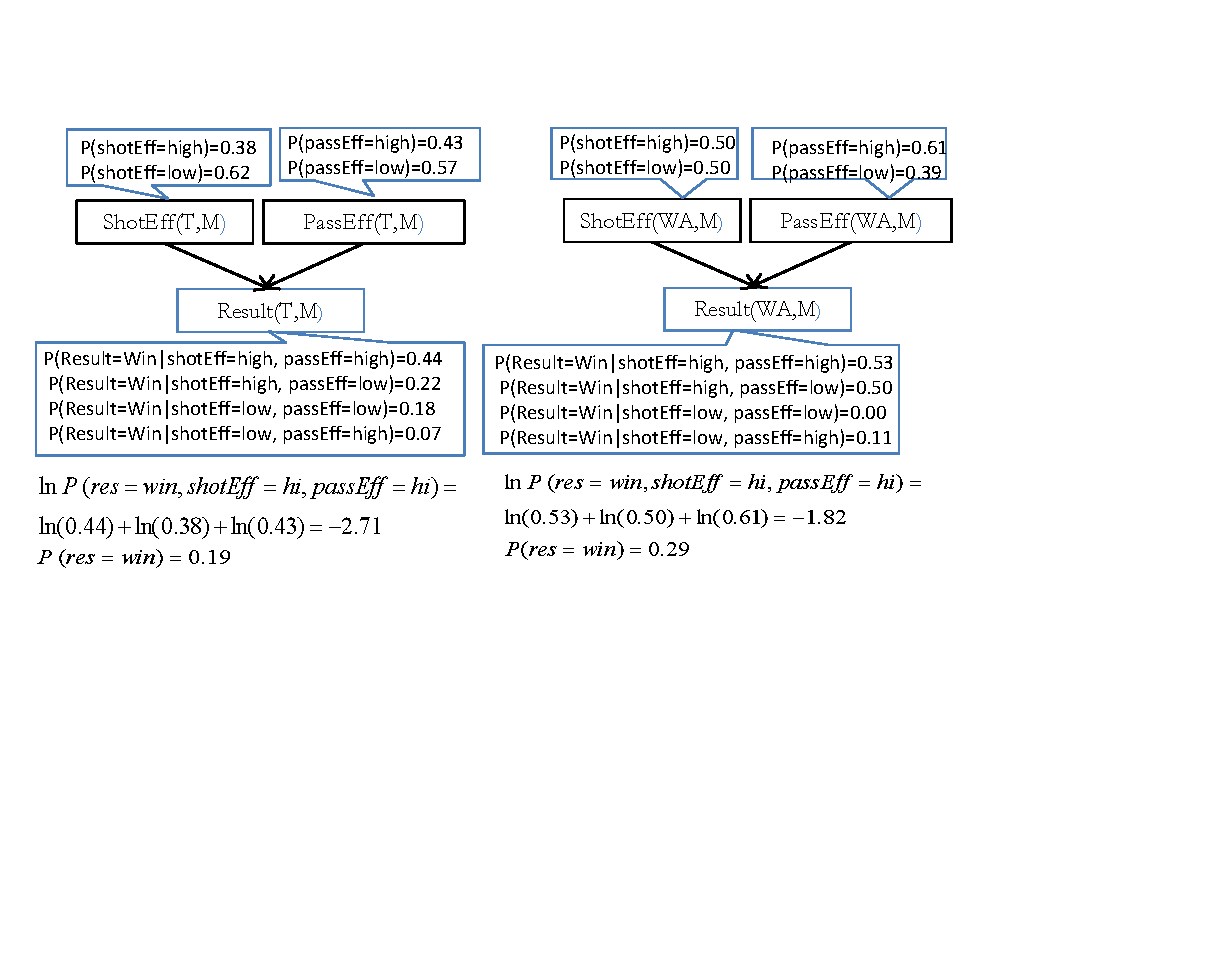
\includegraphics[width=1\textwidth] 
 		{figures/bnuncropped}
 		\caption{Example of joint and marginal probabilities computed from a toy Bayesian network structure. The parameters were estimated from the  Premier League dataset. (Top): A class model Bayesian network $\model_{\class}$ for all teams with class parameters $\parameters_{\class}$. (Bottom): The same Bayesian network structure with object parameters $\parameters_{\object}$ learned for Wigan Athletics ($T = WA$). Our model-based methods outlier scores compare the data likelihood of the class parameters and the object parameters.
 			%We show only the Markov blanket of the Results node to simplify. 
 			\label{fig:bns-chap3}
 		}
 	\end{figure}
 	
 
 	
 	%	\begin{figure}[t]
 	%		\centering
 	%		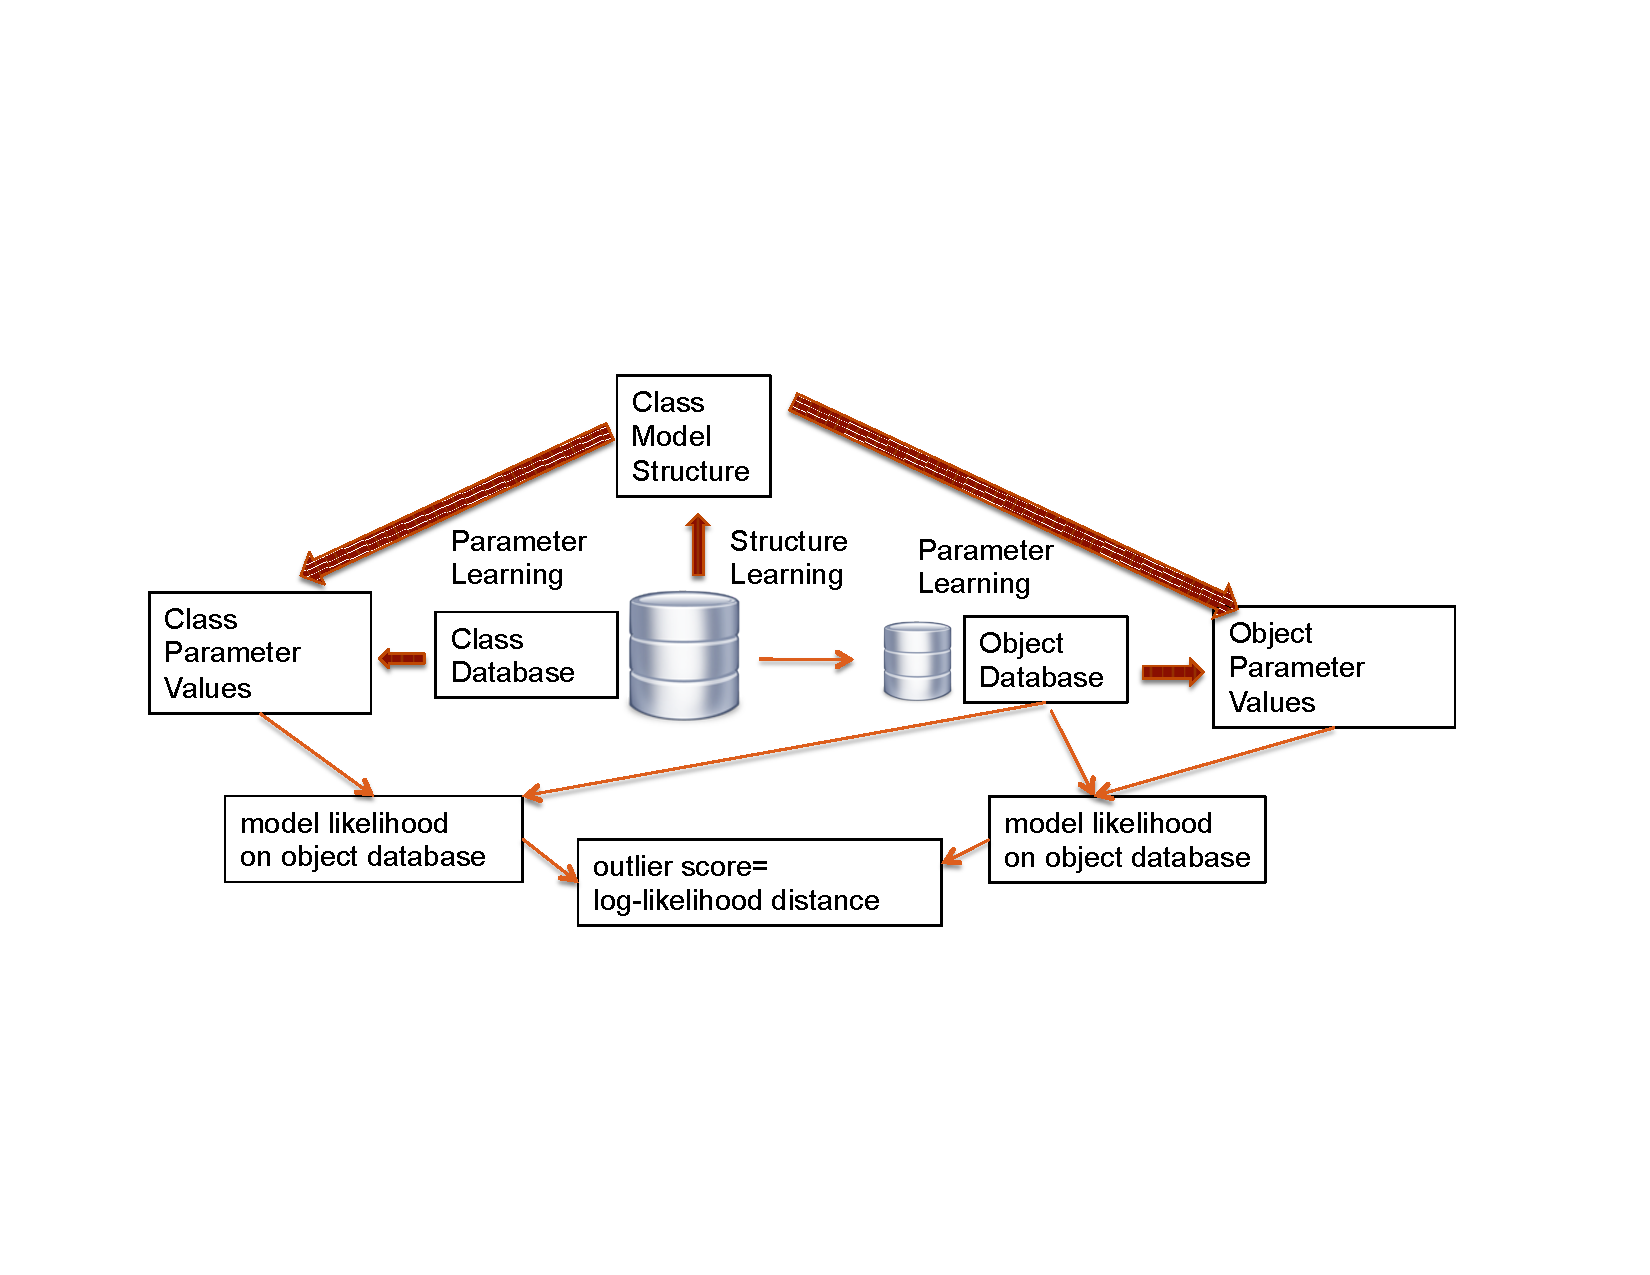
\includegraphics[width=1\textwidth]{figures/flow.pdf}
 	%		
 	%		\caption{Computation of outlier score. 
 	%			\label{fig:flow}}
 	%	\end{figure}
 	%				\begin{figure}
 	%				\centering
 	%				\resizebox{0.9\textwidth}{!}{
 	%				
 	%				\subfigure{
 	%				  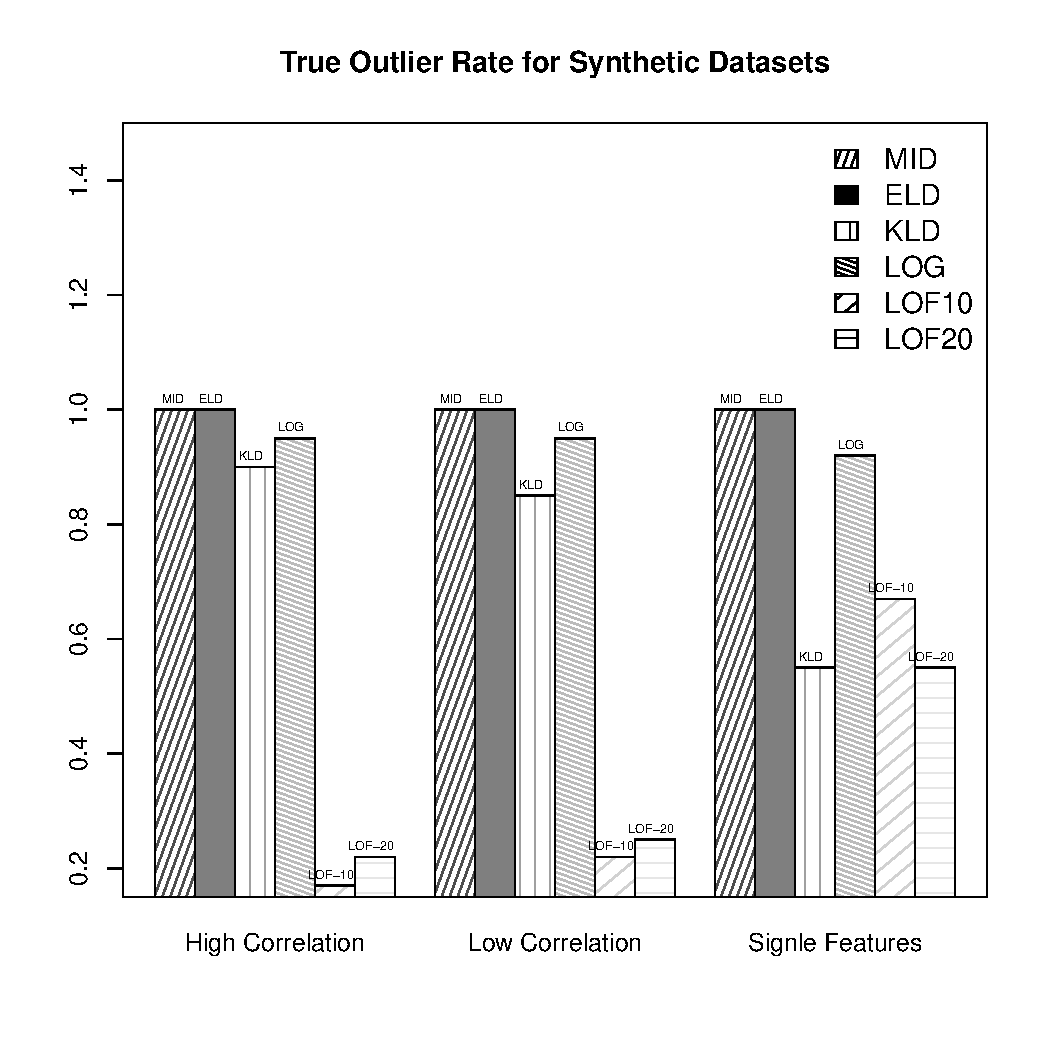
\includegraphics[height=70mm, width=70mm] {figures/TPR-Synthetic.pdf}
 	%				}
 	%				\subfigure{
 	%				  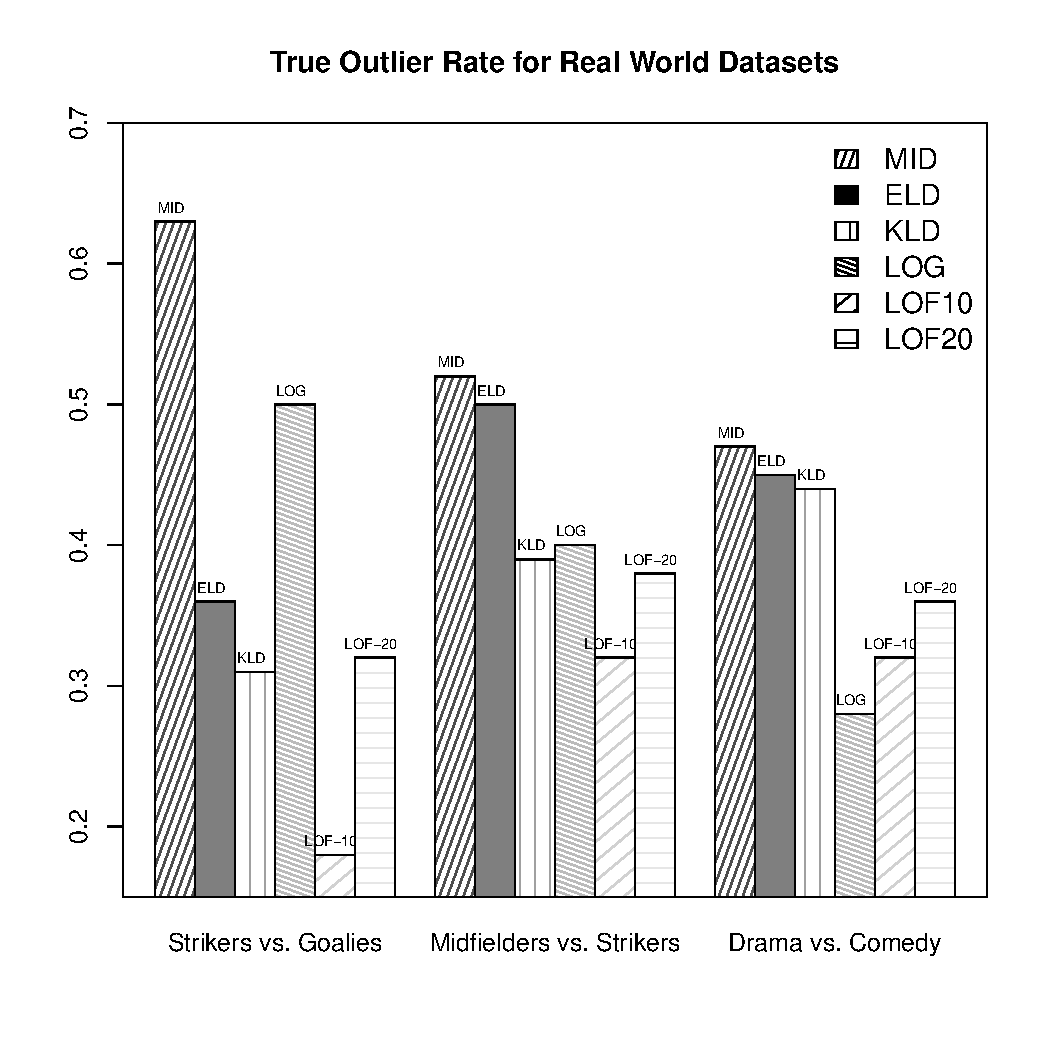
\includegraphics[height=70mm, width=70mm] {figures/TPR-All.pdf}
 	%				
 	%				 }
 	%				 }
 	%				
 	%				\caption{Comparison of Object Outlier Metrics}
 	%				\label{fig:synthetic}
 	%				\end{figure}
 	%				
 	
 	%				\begin{figure}
 	%					\centering
 	%					\begin{subfigure}{0.4\textwidth}
 	%						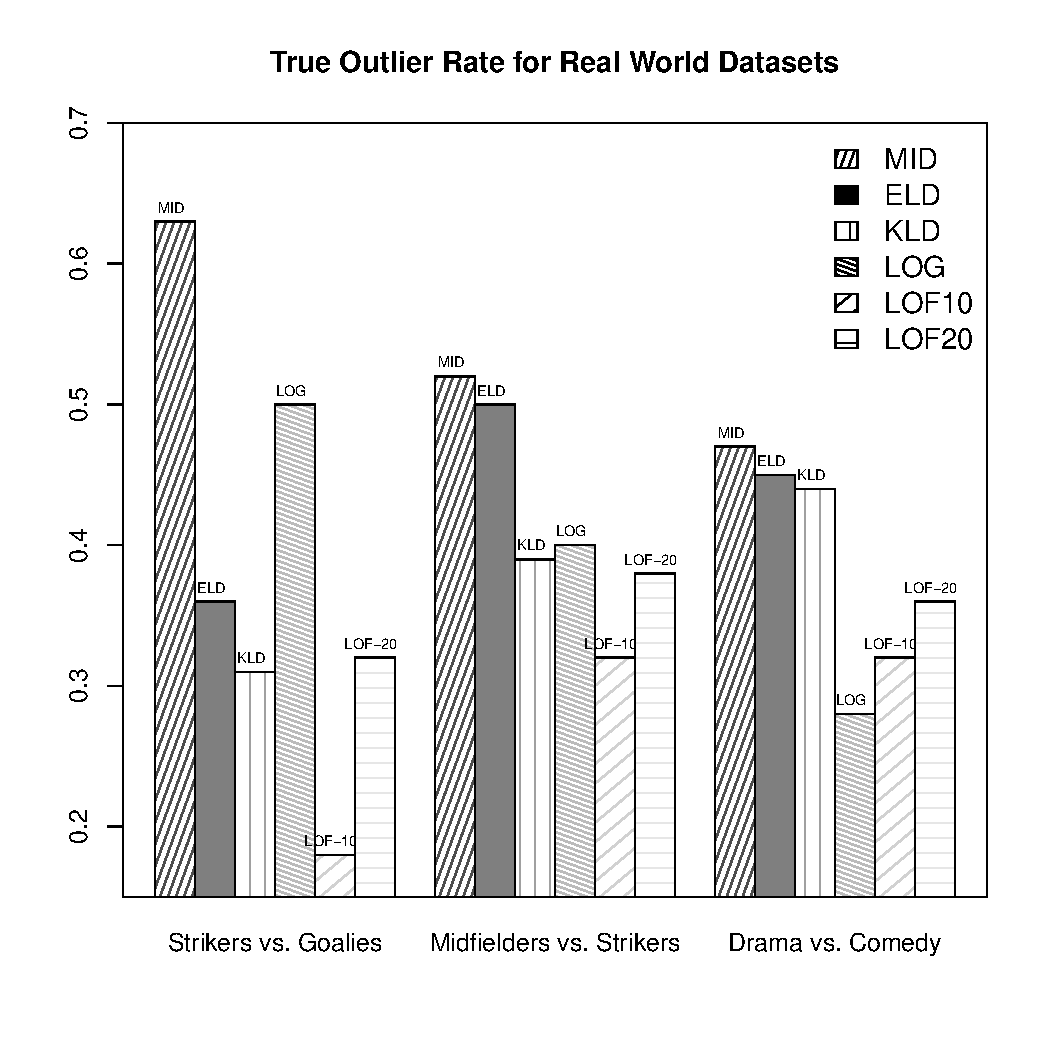
\includegraphics[width=1\linewidth]{figures/TPR-All.pdf}
 	%						\caption{}
 	%						\label{fig:Ng1} 
 	%					\end{subfigure}
 	%					
 	%					\begin{subfigure}{0.4\textwidth}
 	%						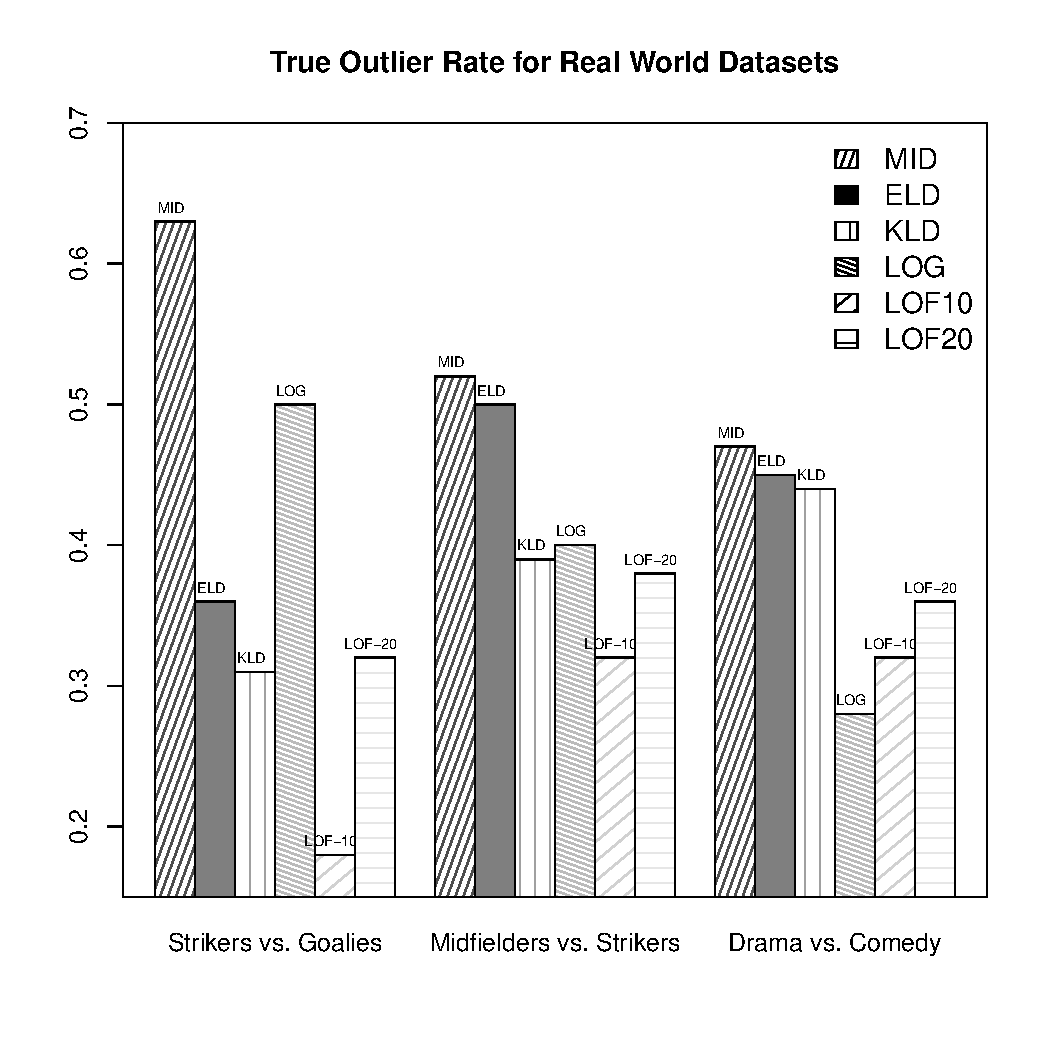
\includegraphics[width=1\linewidth]{figures/TPR-All.pdf}
 	%						\caption{}
 	%						\label{fig:Ng2}
 	%					\end{subfigure}
 	%					
 	%					\caption[Two numerical solutions]{(a) Numerical solutions for the small-time system 
 	%						with a constant-curvature body shape showing the scaled leading-order veritcal 
 	%						reaction force $N_0$ versus the scaled body mass $M$ for various values of $g$. 
 	%						Again, $I=M$ for definiteness and $A=0.7$. (b) As for (a) but over a wider range of 
 	%						values of $M,I$.}
 	%				\end{figure}
 	
  				%			\end{table}
 				
 				%[Example of counts, frequencies]
 				% For simplicity only, suppose that the only matches and players in the season are those shown in Table~\ref{table:data}. Then the attribute value $\it{First\_goals} = 0$ occurs with frequency $1/2$ in the object distribution $P_{\it{si}}$ for Silca. In the player class distribution $P_{\it{Player}}$, the attribute value $\it{First\_goals} = 0$ occurs with frequency $4/5$. So Silva is somewhat less likely to score no goal than a randomly selected player.
 			%	\subsubsection{Bayesian Networks for Relational Data}
 				
 
 				%For most of the paper we refer to PBNs simply as Bayesian networks, and to PRVs simply as random variables. 
 				%The learn-and-join algorithm is the state-of-the-art Bayes net learning method for relational data, based on model search in the lattice of relationship joins \cite{Schulte2012}. The LAJ algorithm takes as input a relational database and outputs a Parametrized Bayes net structure.
 				%We review the algorithm very briefly; for further details please see \cite{Schulte2012}. 
 				%The algorithm builds a Bayes net for an entire database by level-wise search through the {\em lattice of relationship chains.} This is the lattice of relationship sets that are connected by shared first-order variables.
 				%%; see Figure~\ref{fig:lattice}.  
 				%%We describe the fundamental ideas of the algorithm; for further details please see \cite{Schulte2012}. 
 				%The user chooses a single-table Bayes net learner. The learner is applied to base population data tables. Then the learner is applied to data tables for relationship chains of size $s,s+1,\ldots$, with the constraint that the models for larger join tables inherit the absence or presence of learned edges from smaller join tables. 
 				%

 				

 				% shows a sample PBN.
 				
 				
 				%We use the following notation.
 				
 				%\begin{figure}[ht]
 				%\centering
 				%   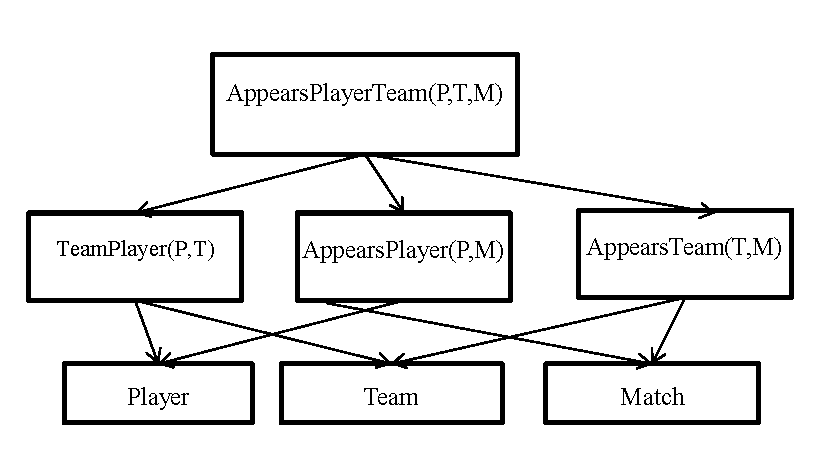
\includegraphics[width=0.3\textwidth] {lattice}
 				% \caption{Lattice of Premier League dataset.
 				% %We show only the Markov blanket of the Results node to simplify. 
 				% \label{fig:lattice}}
 				%\end{figure}
 				
 				
 				
 				
 				%\begin{itemize}
 				%\item $\D_{\population}$ is the database for the entire population; cf. Table~\ref{table:data}.
 				%\item $\D_{\target}$ is the restriction of the input database to the target object; cf. Table~\ref{table:object}. 
 				%\item $\M_{\population}$ is a model (e.g., Bayesian network) learned with $\D_{\population}$ as the input database; cf. Figure~\ref{fig:bns}(a).
 				%\item $\M_{\target}$ is an object model (e.g., Bayesian network) learned with $\D_{\target}$ as the input database; cf. Figure~\ref{fig:bns}(b).
 				%\end{itemize}
 							
 %	\subsection{Logical Concepts}
% 	We follow the description of propositionalization in Lippi {\em et al.} \cite{Lippi2011}, where the input to a propositionalizer is a relational database, and the output is a pseudo-\iid data view. 
% 	We adopt a term-based notation for logical concepts~\cite{Poole2003,Chiang2012}. Constants such as $\it{rooney}$, $123$ are used to represent individuals.
% 	% A \textbf{population} is a set of individuals. 
% %	A functor is a function or predicate symbol, denoting a function that is applied to individuals. Each functor has a set of possible values (constants) called the \textbf{domain} of the functor. The domain of a \textbf{predicate} is $\{\true,\false\}$. Predicates are usually written with uppercase Roman letters, other terms with lowercase letters.
% 	
% 	A predicate of arity at least two is a \textbf{relationship} functor. Relationship functors specify which objects are linked. Other functors represent \textbf{features} or \textbf{attributes} of an object or a tuple of objects (i.e., of a relationship).
% 	A \textbf{term} is of the form $f(\term_{1},\ldots,\term_{k})$ where $\functor$ is a functor %(either a function symbol or a predicate symbol) 
% 	and each $\term_{i}$ is a first-order variable or a constant. 
% 	An {\em atomic assignment} specifies the value of a term e.g. $\functor(\term_{1},\ldots,\term_{k})=v$ where $v$ is in the domain of functor $\functor$. 
% 	%A literal is also a {\em formula}. 
% 	%		Formulae with multiple literals are formed using connectives $\wedge$ and or $\vee$. 
% 	Connecting assignments using only $\wedge$ forms a {\em conjunctive formula } or {\em conjunction}. In this dissertation we use conjunctive formulas only. A term/literal/formula is \textbf{ground} if it contains no first-order variables; otherwise it is a first-order term/literal/formula. 
% 	
% 	An object-relational database $\D$ specifies the values of all ground terms, and hence whether a ground literal is true or not. A ground conjunction is true in a database if all of its conjuncts are true.
% 	% A \textbf{grounding} is a set $\{X_{1} \backslash x_{1}, \ldots, X_{k}\backslash x_{k}\}$ where $X_{i}$ are distinct logical variables and $x_{i}$ are constants. When applied to a formula, each occurrence of $X_{i}$ is replaced with $x_{i}$. 
% 	%We denote the application of a substitution 
% 	%$\{X_{1} \backslash x_{1}, \ldots, X_{k}\backslash x_{k}\}$ 
% 	%		to $f$ as $f\{X_{1} \backslash x_{1}, \ldots, X_{k}\backslash x_{k}\}$.
% 	%		
% 	The count of groundings that satisfy (make true) formula $\formula$ with respect to a database $\D$ is denoted as $\grounds_{\D}(\formula)$.	
 	
 	
 	\subsection{Markov Logic Network} A Markov Logic Network (MLN) \cite{Domingos2009} is a set $\{(\formula_{1},\w_{1}),\ldots,(\formula_{\numformulas},\w_{\numformulas})\}$ where $\formula_{i}$ is a formula, and each $\w_{i}$ is a real number called the weight of $\formula_{i}$. The MLN semantics views a formula with logical variables as a feature template that is instantiated by ground formulas. The number $\numformulas$ of formulas is independent of the size of the instantiated MLN.
 	The log-linear likelihood of a possible world/database is proportional to the weighted sum, over all formulas, of the grounding count of each formula in the given database:
 	\begin{equation} \label{eq:mln} P(D) \propto \exp(\sum_{i=1}^{\numformulas} \w_{i} \cdot \grounds_{\D}(\formula_{i}))\end{equation}
 	
 	This semantics defines a joint distribution over descriptive attributes of entities, links between entities, and attributes of those links. Domingos {\em et al.} discuss the representational power of this semantics~\cite{Domingos2009}. %Table~\ref{MLNFormulas} shows an MLN for the Soccer domain.
 	%

 		
% 		\begin{table}
% 			\centering
% 			\begin{tabular}
% 				{|l|l|l|} \hline
% 				First-order logic  & Weight& English \\ \hline
% 				\multirow{2}{*} {$\forall x ($\textit{shotEfficiency}$(x) \Rightarrow$ \textit{dribbleEfficiency}$(x))  $} & \multirow{2}{*} {$w_1$} & if shot efficiency of the player is \\ & &high then  dribble efficiency is high \\ \hline
% 		%		$\forall x \forall y (intelligent(x) \wedge  friend(x,y)$ & \multirow{2}{*}{ 0.7}& If a student has an intelligent \\ $\Rightarrow$ $intelligent(y)$) & & friend then he is intelligent  \\ \hline
% 			\end{tabular}
% 			\caption{Example of a small MLN }
% 			\label{MLNSample}
% 		\end{table}
 		
\begin{table*}
	
	\centering
	\caption{ MLN formulas derived from the toy Bayesnet shown in Figure~\ref{fig:bns-chap3} 
		\label{table:MLNFormulas}}
	\resizebox{1\textwidth}{!}{
		
		\begin{tabular}{c}
			\hline
			%Formula&\multicolumn{2}{|c|}{\begin{tabular}{p{5cm}} $1/2 \log(0.5/0.5)=0 $\end{tabular}}\multicolumn{2}{|c|}{F2 Vector}\\\hline
			Formula\\\hline
\begin{minipage}{15cm}\begin{equation} \it{Result(T,M)}=win\wedge \it{ShotEff(P,M)}=high\wedge \it{\it{PassEff}}(P,M)=high \nonumber\end{equation}\end{minipage} \\\hline
\begin{minipage}{15cm}\begin{equation} \it{Result(T,M)}=win\wedge \it{ShotEff(P,M})=high\wedge \it{\it{PassEff}}(P,M)=low \nonumber\end{equation}\end{minipage} \\\hline
\begin{minipage}{15cm}\begin{equation} \it{Result(T,M)}=win\wedge \it{ShotEff(P,M)}=low\wedge \it{\it{PassEff}}(P,M)=low \nonumber\end{equation}\end{minipage} \\\hline
\begin{minipage}{15cm}\begin{equation} \it{Result(T,M)}=win\wedge \it{ShotEff(P,M)}=low\wedge \it{\it{PassEff}}(P,M)=high \nonumber\end{equation}\end{minipage} \\\hline
\begin{minipage}{15cm}\begin{equation} \it{ShotEff(P,M)}=high \nonumber\end{equation}\end{minipage} \\\hline
\begin{minipage}{15cm}\begin{equation}\it{ShotEff(P,M)}=low \nonumber\end{equation}\end{minipage} \\\hline
\begin{minipage}{15cm}\begin{equation}\it{PassEff(P,M)}=high \nonumber\end{equation}\end{minipage} \\\hline
\begin{minipage}{15cm}\begin{equation}\it{PassEff(P,M)}=low \nonumber\end{equation}\end{minipage} \\\hline
 %\parbox{10cm}{\begin{equation} SavesMade(P,M)=med\wedge shotsOnTarget(P,M)=lo\wedge \it{\it{ShotEff}}(P,M)=lo \nonumber\end{equation}}&2\\\hline

		\end{tabular}
	}
	
\end{table*}
 	\subsection{Structure Learning} In this dissertation, for Bayesian network structure learning we employ the Learn-and-Join (LAJ) algorithm. This is a state-of-the-art structure learning algorithm, especially well-suited for datasets with many descriptive attributes such as those we used in our evaluation \cite{Khosravi2010,Schulte2012}. 
 	
 	 The LAJ algorithm employs an iterative deepening strategy, which can be described as follows for object data. The algorithm learns a set of interrelated BNs. The initial step is to learn one BN for each object class. The BN for one class represents associations among the features of the objects in the class only. The algorithm then learns a BN for
 	 each pair of linked components, such that the BN for the pair inherits the edges of the BNs for the objects.
 	 Next, the algorithm learns a BN for each triple of objects related by a path of length 2, where edges are inherited
 	 from the BNs for the relevant pairs, etc. The algorithm stops when increasing the path length leads to no new
 	 edges being learned. The multiple Bayesian networks are then merged into complete Bayesian networks for
 	 all objects. The LAJ algorithm takes as input a relational database and outputs a Parametrized Bayes net structure.
 	 
 	 The Parametrized Bayes net learned from LAJ algorithm can then be converted to an MLN set of clauses using the moralization method described by Domingos and Richardson\cite{Domingos07}. Moralization converts the probabilistic clauses defined by Bayes net to conjunctions of literals as shown in Figure~\ref{MLNLearningProcess}. An example of this conversion is shown in Table~\ref{table:MLNFormulas}.
 	 
 	 
 	  	\begin{figure}[t]
 	  		\centering
 	  		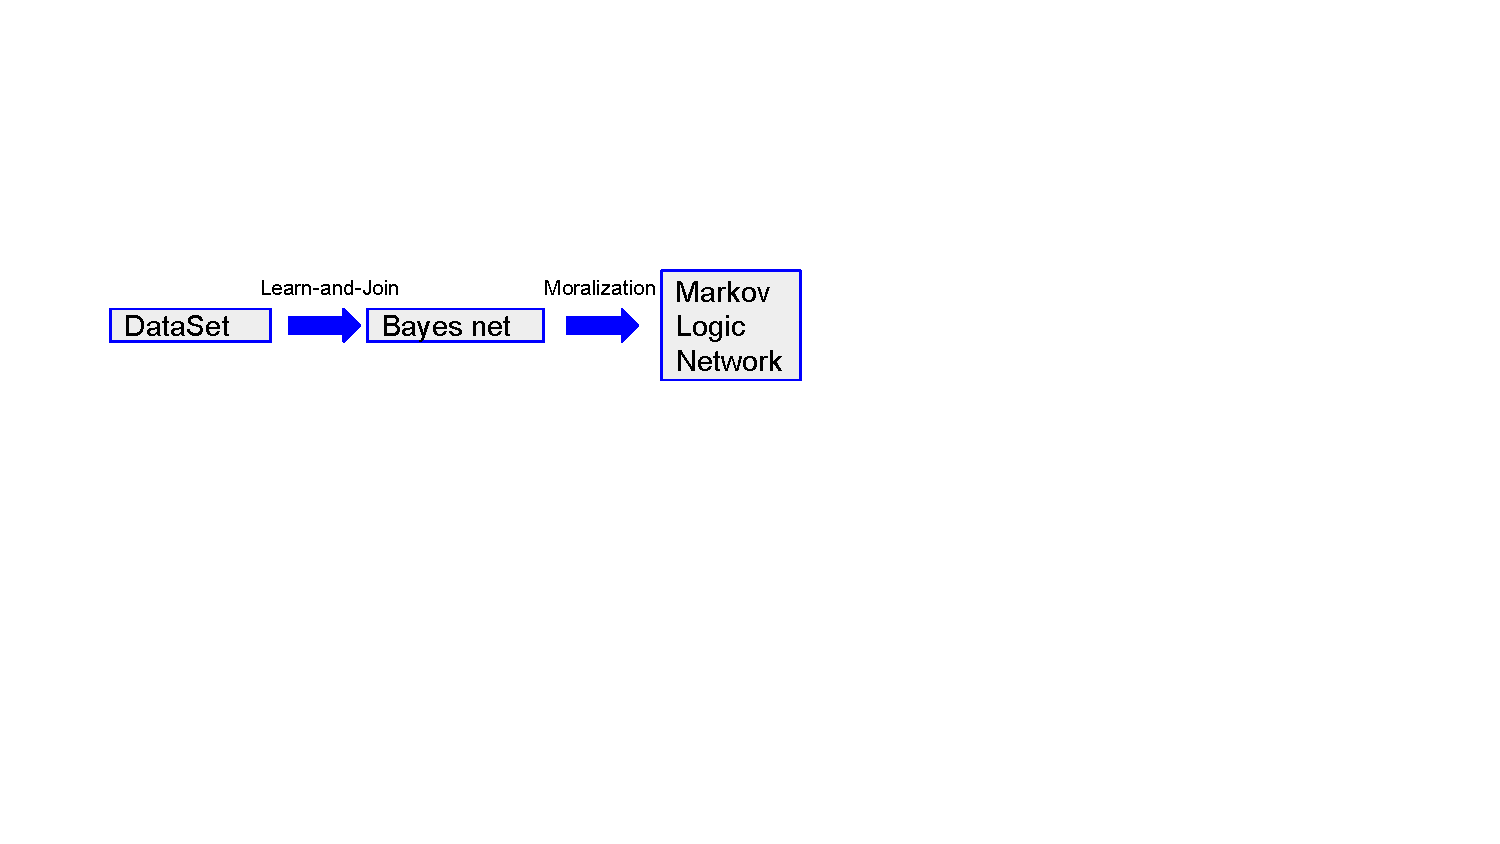
\includegraphics[width=0.8\textwidth] 
 	  		{figures/MLNLearningProcess.pdf}
 	  		\caption{Learning an Markov Logic Network from an input relational database.
 	  			%We show only the Markov blanket of the Results node to simplify. 
 	  			\label{MLNLearningProcess}
 	  		}
 	  	\end{figure}
 	 
 %	figures/MLNLearningProcess.pdf
%	 The LAJ algorithm employs an iterative deepening strategy, which can be described as as search through a lattice of table joins. For each table join, different BNs are learned and the learned edges are propagated from smaller to larger table joins. 	For a full description, complexity analysis, and learning time measurements, please see \cite{Schulte2012}. 	We used the implementation of the LAJ algorithm due to its creators \cite{bib:jbnsite}. 
 	
% 	Our emphasis is on comparing {\em learning} formulas with the baseline of {\em enumerating} all $n$-grams, so we leave for future work
% 	evaluating other MLN structure learning algorithms, such as MLN-Boost \cite{Khot2011}. 	% rather than different versions of the MLN approach. 
 	%In direct comparisons between the LAJ and the MLN-Boost systems, the classification accuracy of LAJ models has been competitive with those found by MLN-Boost~\cite{Schulte2012d}. 
 	
 	%We briefly describe the Learn-and-Join algorithm (LAJ). 
% 	The LAJ algorithm has also been employed  for MLN structure learning task. it distinguishes between descriptive attributes, such as $\it{gender(User)}$ or $\it{Rating(User,Movie)}$ and relationships, such as $\it{HasRated}(\it{User},\it{Movie})$. Relationships indicate the existence of a certain type of link between individuals. 
% 	%Attributes are properties of individuals or links. Both can be represented using  atoms. 
% 	A relationship chain is a list of relationship atoms connected by shared logical variables. 
% 	%The LAJ algorithm carries out a lattice search that performs iterative deepening with relationship chains of increasing depth. 
% 	Note that for every relationship atom, there is a set of associated descriptive attributes. For example, for the predicate $\it{HasRated}(\it{User},\it{Movie})$, the associated attributes comprise the rating, as well as the descriptive attributes of users and movies. For the initialization, for each relationship atom, the algorithm learns a set of formulas for the attributes associated with that relationship. In the implementation of \cite{Schulte2012}, a propositional graphical model learner is used to find the set of formulas. For a relationship chain of length $\ell +1$, the algorithm learns another set of formulas for the attributes associated with the relationships in the chain, with the following constraint: all formulas discovered for subchain of length $\ell$ or less are inherited by larger relationship chains. %LAJ algorithm can also be used to learn MLN structure. 
 	
 	
 	%%				
 	%%				\subsubsection{Examples} Figure~\ref{database} shows an example database. The ground literal $$(\it{ShotEff(\P,\M)} = Low) \{\P\backslash 123,\M\backslash 1\}$$$$=(\it{ShotEff}(123,1)=Low)$$ evaluates as true in this database. For the grounding count we have $$\grounds_{\D}(\it{ShotEff(\P,\M)} = Low) \{\P\textbackslash 123\}) = 2.$$
 	%%				
 	
 	%
 	%how much more general a learned rule set is if anomalous examples are omitted either by measuring the difference of the generalization of the hypotheses induced in presence or absence of the observation~\cite{Angiulli2009} or by means of satisfaction of certain conditions~\cite{Angiulli2004}. 
 	
 	
% 	\begin{figure}
% 		\centering
% 		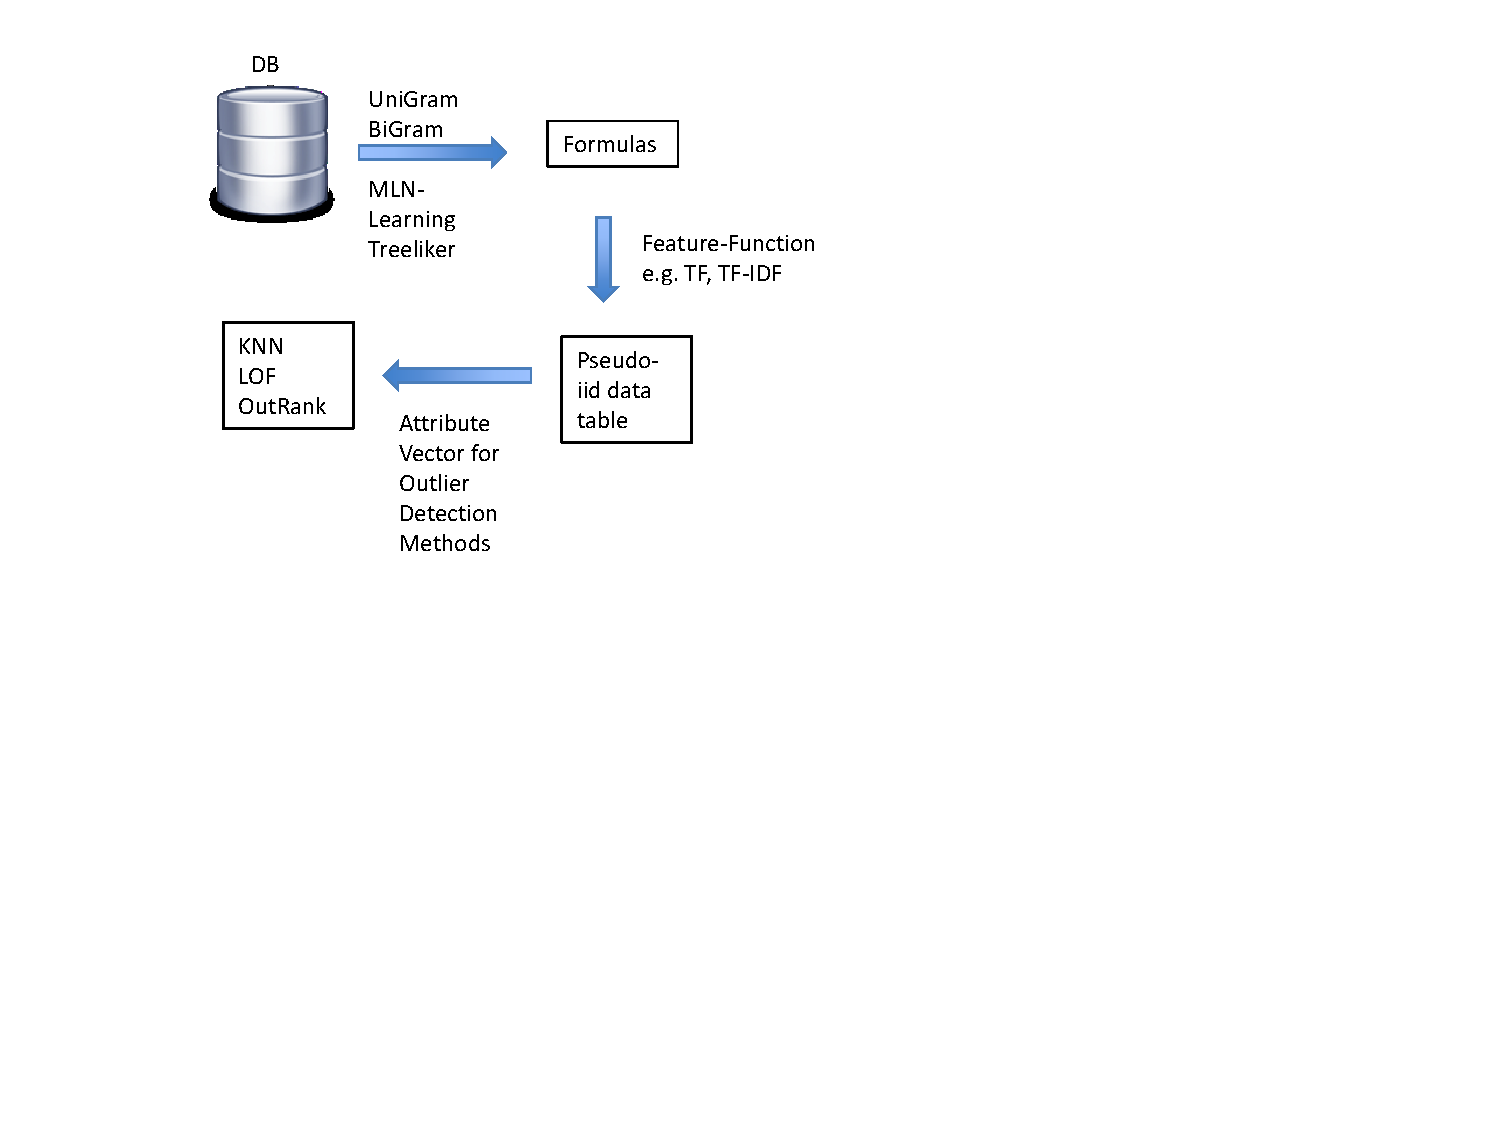
\includegraphics[width=0.6\textwidth] {figures/OverView.pdf}
% 		\caption{System Flow
% 			\label{main:b-chapter3}}
% 	\end{figure}
% 	
 
\section{Evaluation Techniques in Outlier Detection}\label{sec:eval}
Measuring the effectiveness of outlier detection methods is not often an easy task. Most of the time ground truth information, that shows which data points are outliers, is unavailable. \\
%In this section, we first discuss how outlier detection methods in the literature have tackled this problem, then we describe how we deal with it in our research.\\ 
Several techniques have been employed in literature to evaluate the performance of outlier detection methods:
\begin{enumerate}
\item Intuitive evaluation: case studies have been extensively used in literature to evaluate outliers~\cite{aggarwal2013}. In chapter 4 we use this method of evaluation for top $n$ ranked detected outliers and we try to explain and make sense of the detected outliers. 	
\item Synthetic data generation: another approach to evaluate anomaly detection methods is generating synthetic data and inject synthetic outliers into the data~\cite{aggarwal2013}. We have designed and developed three synthetic datasets as it was discussed in section~\ref{sec:synthetic}.
\item Anomaly injection: anomalies are injected into the real-world datasets. Outlier detection methods are expected to detect the injected data points as outliers~\cite{Akoglu2015}. We employ this approach in our real world datasets.
The disadvantage of this evaluation metric is that the real world data may also contain certain type of anomalies, known as in-class outlier. However, this metric treats only the injected data points as true positive and will score anything other than those as false positive.
\item Internal Evaluation: in this type of evaluation outlier score has been used to quantify the extremity of data points~\cite{Pickands1975}.% We do not use this method of evaluation in our work.
\end{enumerate}





